\documentclass[a4paper,11pt]{article} % Artículo porque a la hora de poner los títulos los enumera con 1., 2.,... sin embargo el report te los enumera así: 0.1., 0.2.,...
\usepackage[utf8x]{inputenc} % Esto hace que latex interprete la codificación del documento como utf-8 sin dar errores en las tildes
\usepackage[spanish]{babel} % Para poner el idioma en castellano(fecha,Índice...)

%Estas dos líneas (esta y la de abajo)ponen interlineado 1,5 excepto en notas a pie de página e igual algo más (que no sé)
\usepackage{setspace} % Paquete para interlineado.
\onehalfspacing % Interlineado a 1'5

\usepackage{helvet}
\renewcommand{\familydefault}{\sfdefault}
%\usepackage{uarial}
%\renewcommand{\familydefault}{\sfdefault}

\usepackage[top=2.5cm, left=4cm, bottom=2.5cm, right=3cm]{geometry} % Para los márgenes

\usepackage{color} % Para poder poner las letras en color si es necesario
\usepackage[toc,page]{appendix} % Para poder poner los Anexos
\renewcommand{\appendixname}{Anexos} %Para cambiar de nombre los appendices por anexos
\renewcommand{\appendixtocname}{Anexos} %Para cambiar de nombre los appendices por anexos
\renewcommand{\appendixpagename}{Anexos} %Para cambiar de nombre los appendices por anexos


\begin{document} % Siempre hay que ponerlo
\title{Anatomía de superficie: su representación pictórica en el Ecce Homo}
\author{Nerea González Cordero}
\date{\today}
\maketitle % Para crear la portada
\thispagestyle{empty} % Para que no ponga número en la página
\newpage % Para salto de página

\pagestyle{empty}
\tableofcontents % Para el Índice
\newpage
\pagestyle{plain}
\pagenumbering{arabic} % La numeración de las páginas, también se puede con números romanos {roman}

\section{Introducción} % Para los títulos
El arte podría definirse como una expresión de la creatividad humana que produce obras apreciadas por su belleza o emotividad y que es innata en el ser humano \footnote{Definición según el Diccionario Oxford: www.oxforddictionaries.com/definition/english/art}. Existe desde el origen del ser humano y  % (http://www.oxforddictionaries.com/definition/english/art)
a lo largo de los siglos ha ido evolucionando hasta el arte contemporáneo. Junto con las obras artísticas también se han ido transformando las representaciones anatómicas en las obras pictóricas y escultóricas.

La anatomía de superficie es la ciencia que estudia las características anatómicas que pueden ser estudiadas mediante la vista y la palpación \footnote{Definición según Wikiradiography: www.wikiradiography.com/page/Surface+Anatomy}% (http://www.wikiradiography.com/page/Surface+Anatomy)
, es decir, la superficie del cuerpo. En el caso de la anatomía humana estudia desde las proporciones del cuerpo hasta puntos de referencia visibles en el exterior que están relacionados con órganos y partes internas, tanto en pose estática como en movimiento. % (http://www.princeton.edu/~achaney/tmve/wiki100k/docs/Superficial\_anatomy.html)
% %http://www.theodora.com/anatomy/surface\_anatomy\_index.html

%Como la materia principal de mi trabajo es la antomía de superficie relataré lo más relevante acerca de cómo ha evolucionado el conocimiento de esta materia hasta llegar al conocimiento actual.
\subsection{Historia de la anatomía}
A lo largo de la historia ha habido diferentes impedimentos que han provocado que hasta épocas muy recientes la anatomía del cuerpo humano fuese una gran desconocida, incluso entre aquellos que fundamentalmente trabajaban vinculados al cuerpo humano por distintas razones, como pueden ser médicos o artistas.

Desde el antiguo Egipto se ha estudiado la anatomía del ser humano, aunque no estaba a la altura del desarrollo médico que poseían, posiblemente por el gran respeto que profesaban a los cadáveres. Conocían algunas estructuras como el corazón, el cual consideraban el órgano central y lugar del pensamiento y los sentimientos, el hígado, el bazo, los riñones e incluso la existencia de vasos sanguíneos que transportaban distintos fluidos.

Los griegos fueron los grandes anatómicos de la antigüedad, de hecho, se recogen bastantes textos médicos en el Corpus Hipocraticum \footnote{Colección de trabajos médicos elaborados en la antigua Grecia. A pesar de su nombre no está comprobado que Hipócrates sea el autor de todos estos escritos, de hecho se desconoce el autor de la mayoría de ellos.}. En estos se describen la función de algunos órganos, así como del sistema músculo-esquelético y también la diferencia entre arterias y venas. Fueron los primeros en formar escuelas de anatomía e incluso los primeros en diseccionar cuerpos humanos \footnote{Ptolomeo I fue el primero que aprueba la utilización de cuerpos humanos para su disección y estudio anatómico. Durante su reinado y el de su dinastía fue posible para algunos anatomistas la realización de disecciones. El más importante es Herófilo considerado como "Padre de la anatomía".}, lo que permitió un conocimiento más avanzado del cuerpo humano. Sin embargo, esto no era lo habitual y normalmente utilizaban sus conocimientos de las disecciones de animales para aplicarlos a la anatomía humana.

Galeno siguió con los estudios anatómicos mediante la disección de animales aportando además otros conocimientos que recibía gracias a su condición de médico entre los gladiadores donde podía vislumbrar cualquier tipo de herida. Sus estudios se encuentran recogidos en sus numerosos tratados. \footnote{Galeno con más de 500 tratados fue el autor de la antigüedad que más escritos elaboró.}

En otras culturas como la india y la china la anatomía tampoco estaba más desarrollada que la occidental, que se basó durante varios siglos en los tratados galénicos.

El conocimiento anatómico del ser humano apenas avanzó en occidente durante la Edad Media, debido a la creencia cristiana de que el alma de un cuerpo diseccionado no podría ir al ``Cielo". Por ello las disecciones fueron un tema tabú durante esta época, y desapareció el interés por el cuerpo concentrándose éste en el alma. La cultura islámica poseía un conocimiento médico muy desarrollado para la época, sin embargo las disecciones de cadáveres humanos estaban prohibidas, por lo que su conocimiento de anatomía se basaba en las disecciones de animales y no era muy superior al de la Europa cristiana.

%Posteriormente, ya en la Edad moderna, se conceden permisos para diseccionar cadáveres de criminales como una parte más de la pena por su delito.

No es hasta Leonardo Da Vinci que se empezaron a hacer verdaderos progresos en la anatomía humana. Sus conocimientos se debieron a disecciones que llevó a cabo en cuerpos humanos y están plasmadas en una gran variedad de dibujos \footnote{El Hombre de Vitruvio es la más conocida de todas las ilustraciones elaboradas por Da Vinci (ver anexo \autoref{app:vitruvio}).}. Aunque el verdadero cambio de la anatomía galénica a una doctrina más moderna se dio en el siglo XVI gracias a Andrés Vesalio. Éste es el autor de "De Humani Corporis Fabrica", donde se recogen diversos dibujos de anatomía humana (ver anexo \autoref{app:vesalio}). Vesalio, junto con otros personajes influyentes de la época y posteriores como Miguel de Servet o William Harvey, provocó una auténtica revolución en la anatomía tradicional.

%Además, a partir de este momento los estudiantes de anatomía no tenían que saber latín para poder estudiar y lo podían hacer mediante las diversas representaciones que se estaban llevando a cabo.

Las disecciones empezaron a ser más comunes, y se observaron varios problemas.

El primer problema se debía a la temperatura del ambiente. En aquella época no se conocía la manera de conservar un cuerpo. Es por esto que la disecciones se podían realizar exclusivamente en los meses de temperatura más baja, cuando el frío mantenía el cadáver por más tiempo. Aún así había que realizar la disección casi inmediatamente después de la muerte del individuo, pues los cuerpos no tardaban mucho en descomponerse.

El segundo problema provenía del aumento de las disecciones. Debido a los pocos cuerpos que  se permitían diseccionar y al aumento de estudiantes de anatomía se empezaron a profanar tumbas para conseguir cadáveres, algunos incluso llegaron más lejos matando a personas para vender sus cuerpos \footnote{Son conocidos los asesinatos de West Port o de Burke y Hare que fueron llevados a cabo durante 1828 en Edimburgo. William Burke y William Hare asesinaron a dieciséis personas y vendieron sus cuerpos al Doctor Robert Knox, quien los utilizaba en sus clases de anatomía. Cuando se descubrieron los crímenes Hare testificó contra Burke quien fue condenado a muerte y después diseccionado.}.

Para evitar este último problema se elaboró la ley de anatomía de 1832 (Reino Unido) que regulaba las donaciones de cuerpos a la ciencia y la obtención de licencias para obtener el permiso que permitía diseccionar cadáveres.

%Durante los siglos XVII y XVIII el campo de la anatomía se desarrolla tremendamente. Al principio se realizaban disecciones en plazas donde cualquiera podía atender a la explicación de un maestro, después, no obstante las disecciones pasan a realizarse en aulas siendo muchos menos los beneficiados que aprendían anatomía.

En los siglos XIX y XX el conocimiento anatómico adquirió su completa madurez gracias al avance de otras disciplinas científicas y tecnológicas que ayudaron a ello.
% http://www.bl.uk/learning/artimages/bodies/vesalius/renaissance.html
% http://www.sciencemuseum.org.uk/broughttolife/themes/understandingthebody/dead.aspx
% http://en.wikipedia.org/wiki/Anatomy\_Act\_1832
% http://en.wikipedia.org/wiki/Cadaver
% http://en.wikipedia.org/wiki/History\_of\_anatomy
% http://en.wikipedia.org/wiki/Hippocratic\_Corpus
% http://en.wikipedia.org/wiki/Galen
% Historia de la anatomía. Dr José Alfredo Sillau Gilone (en descargas 3 partes: libro de historia de la anatomía, historia anatomía e historia de la anatomía.)


\subsection{Muerte de Cristo}
La muerte de Cristo es una tema muy recurrido en la obra pictórica. En los siglos inmediatamente posteriores a la crucifixión no representaban tal cual al Cristo en la cruz, sino que lo hacían mediante otros símbolos y más tarde exclusivamente la cruz. Fue, sobre todo, a partir de la Edad Media (siglo V) cuando empezó a ser frecuente la imagen del Cristo crucificado.

Por otra parte, la iconografía cristiana varía de forma y estilo según las percepciones de la época artística en la que se desarrolla, en la que predomina un estilo determinado, pero en todas ellas ha tenido gran relevancia. De un joven imberbe se pasa a un hombre con barba. Ambas representaciones confluyen, pero artísticamente al final persiste la segunda. También se pasa de una visión de un Cristo triunfal a una visión más humana y menos divina de Cristo en el suplicio de la crucifixión.

Puesto que fue el emperador Constantino quien abolió la crucifixión en el siglo IV d.C, y no hay documentación ni representaciones acerca de ello hasta varios siglos después, es difícil saber cómo era, en la época romana, esta pena capital, que se utilizaba únicamente para los peores delincuentes.

Se sabe que aunque ha habido distintas formas de crucifixión, los romanos del periodo comprendido alrededor del nacimiento y la muerte de Cristo utilizaban la cruz \textit{commisa}, vulgarmente denominada cruz latina que es la más frecuentemente representada, o la cruz \textit{immissa}, en forma de T (ver anexo \autoref{app:crosses}). Éstas estaban formadas por dos tablones de madera: un poste vertical que se insertaba en el suelo, que recibe el nombre de \textit{stipes} y un travesaño horizontal denominado \textit{patibulum}. A veces en la mitad del poste vertical se insertaba un bloque de madera que servía de asiento. También se utilizaba, aunque probablemente posteriormente al tiempo en el que vivió Cristo, un tablón que colocado a la altura de los pies ejercía de apoyo para éstos.

Dependiendo de la altura de las cruces éstas se dividían en la \textit{cruz humilde}, la más habitualmente usada, cuya altura era de unos dos metros y la \textit{cruz sublime}, tan alta que los pies del condenado se encontraban aproximadamente a un metro del suelo. Se cree que Cristo pudo haber sido crucificado en una de estas últimas ya que necesitaron una caña para poder acercarle la esponja con vinagre cuando estaba al borde de la muerte (Mt 27, 48; Mc 15, 36; Jn 19, 29). En este aspecto, muchas de las representaciones que podemos observar de crucifixiones de Cristo podrían ser correctas.

Diversas fuentes dejan claro que los romanos utilizaban clavos para sujetar a los individuos crucificados a la cruz \footnote{Así como los evangelios atestiguan que Jesús fue clavado en la cruz, otros autores coetáneos se refieren también al uso de los clavos en la crucifixión. Ejemplos de ello son Séneca y Tranión. Además, las únicas reglas jurídicas que se conocen desde 1967 referentes a la crucifixión dan a entender que a los crucificados se les clavaba en la cruz.}. Además, la crucifixión variaba según la región y la inventiva del verdugo.

La creencia más extendida actualmente es la de que los clavos eran introducidos a la altura de la línea de flexión  de la muñeca, entre el cúbito y el radio y justo entre estos y los carpos o entre las dos filas de huesos metacarpianos. Se ha llegado a esta conclusión tras haber encontrado hallazgos arqueológicos de esa época que concuerdan con esta teoría y tras la realización de experimentos que apuntan a esta misma conclusión\footnote{El doctor Pierre Barbet realizó una serie de experimentos con cadáveres en los que se demostraba esta teoría.}. Anteriormente se creía que los clavaban en las manos porque así lo establece Juan en su Evangelio (Jn 20, 20-29), sin embargo ha de tenerse en cuenta que, antiguamente, la muñeca se encontraba en lo que se denominaba ``mano", que abarcaba hasta el brazo, lo que ha podido inducir a error durante siglos.

En cuanto a la técnica de clavado de los pies, no está claro si realizaban la inserción de los clavos juntando ambos pies y utilizado para ello un solo clavo, o la fijación de éstos se llevaba a cabo por separado mediante dos clavos. Probablemente los clavos eran insertados entre el segundo y tercer metatarsiano. En las representaciones pictóricas se emplea tanto la imagen de Cristo crucificado mediante tres clavos como mediante cuatro.

Teniendo en cuenta las dificultades en el conocimiento de la crucifixión de Cristo es lógico pensar que en la mayoría de la iconografía referente al tema Cristo es representado según el gusto y estilo de cada autor claramente ubicado en su época.

% Enciclopedia moderna, 11: diccionario universal de literatura, ciencias, artes, agricultura, industria y comercio. Francisco de Paula Mellado (Pág:805-811)
% http://www.frugalsites.net/jesus/crucifixion.htm
% http://mb-soft.com/believe/text/crucifix.htm
% LA CRUCIFIXIÓN Laura RODRÍGUEZ PEINADO (en documentos del TFG)
% http://www.shroud.com/bucklin2.htm

Si existe debate acerca de si Jesús murió verdaderamente en la cruz \footnote{Algunos autores como Margaret y Trevor Lloyd Davies, los mayores defensores, consideran la posibilidad de que Jesucristo no muriese verdaderamente en la cruz. Otro ejemplo de esta hipótesis se encuentra reflejada en el libro \textit{42 días, Análisis forense de la crucifixión y la resurrección de Jesucristo}, de Miguel Lorente.}, aún es mayor el debate existente sobre la presunta causa de su muerte.

Existen varias teorías al respecto:

1) Embolia Pulmonar

2) Rotura cardíaca

3) Trauma de suspensión

4) Asfixia

5) Herida perforante fatal

6) Shock

7) Síncope fatal

8) Arritmia cardíaca

9) Coagulopatía inducida por traumatismos.

Todas estas hipótesis han sido analizadas en profundidad, no llegando, sin embargo, a la conclusión acerca de cuál es la real. Lo que está claro, sin embargo, es que Cristo padeció terribles sufrimientos, los cuales en conjunto pudieron conducirle a su muerte, que se produjo hacia las tres de la tarde tras varias horas en la cruz.

% The Search for the Physical Cause of Jesus Christ's Death Author: W. Reid Litchfield Categories: God and Jesus Christ, Science Journal: 37:4 (en documentos de TFG)
% The crucifixion of Jesus: Review of hypothesized mechanisms of death and implications of shock and trauma-induced coagulopathy (en refworks)
%\section{Proporciones del cuerpo humano} %http://es.scribd.com/doc/30286487/Proporciones-Del-Cuerpo-Humano
A lo largo de la historia han ido cambiando las representaciones del cuerpo humano, ya sea por razones ideológicas, estéticas o de conocimiento anatómico.

El deseo de representar al ser humano perfecto impulsó el estudio de las proporciones del cuerpo humano. Esto hizo que se diesen numerosos intentos por representar al ser humano de proporciones perfectas, pudiendo observar este fenómeno desde la antigüedad, en Egipto y Mesopotamia, hasta el hombre de Vitruvio, fruto de los estudios en este ámbito de Leonardo Davinci, y pasando por numerosas representaciones que reflejan los cánones de distintas épocas (Grecia y Roma, Edad Media; y posteriormente, Edad Moderna y Contemporánea).

%Se define cánon como un patrón concreto que fija las proporciones ideales del cuerpo humano en cuanto a su representación pictórica, en este caso.

La mayoría de los artistas confeccionan su canon del cuerpo humano tomando como referencia la cabeza para elaborar las proporciones del resto del cuerpo.
Según la época y el artista los cánones han ido variando, ya que se adaptan al ideal de belleza de la época, que a su vez tiene su origen en los cambios sociales que acontecen en cada período. En el presente se considera como figura ideal el canon de ocho cabezas de altura. Realmente los seres humanos medimos más cerca de siete cabezas de altura que de ocho. Por ello existen tres cánones para determinar las proporciones de la figura humana: el canon de siete cabezas y media, el canon más realista en cuanto a medidas, que se considera la figura común, el canon de ocho cabezas considerado, como ya he dicho, la figura ideal y el canon de ocho cabezas y media, con el que se representan las figuras heroicas.

En la representación femenina es preciso considerar ciertas diferencias anatómicas como la longitud de la cabeza, menor que la del hombre, que hace que su figura sea más baja; los hombros, que son más estrechos; la cintura, más ceñida; las caderas, más anchas; o el ombligo, que está situado más abajo que el del hombre, al igual que el pecho.

Hay que tener en cuenta que los niños guardan otras proporciones. Aunque durante la infancia estamos en constante crecimiento y es difícil crear un canon exclusivo, sí existen algunos cánones aproximados: de cinco cabezas para niños de dos años, de seis cabezas entre seis y doce y de siete entre los doce y los quince.

%http://es.scribd.com/doc/58358634/Canon-de-La-Figura-Humana
\section{Objetivos}
Los objetivos a cumplir en este trabajo son varios. Existe un objetivo principal y otros secundarios.

El objetivo principal será identificar y estudiar la anatomía de superficie en la muerte de Cristo. Para ello se utilizarán varias obras diferentes cuyo análisis nos mostrará la agonía y muerte de Cristo representadas en diferentes épocas que, influenciadas a su vez por el contexto social y religioso, influyen en la pintura o escultura, en la anatomía y en la visión de Cristo de cada época.

Otros objetivos secundarios, relacionados con éste, son: afianzar los conocimientos anatómicos y desarrollarlos, analizar la historia de la anatomía que nos ha permitido llegar al conocimiento anatómico actual e identificar los cambios que se producen en el cuerpo en la agonía y en el momento del fallecimiento y cómo lo han representado en las distintas obras que se analizarán.

Además existen varios objetivos transversales que tienen que ver con la adquisición y la consolidación de conocimientos y habilidades para la realización del Trabajo de Fin de Grado (TFG). Me refiero, en concreto, a: la utilización de las bases de datos de investigación para conseguir información, el desarrollo de la capacidad de síntesis, el análisis crítico de la información encontrada y la elaboración adecuada y estructurada de un TFG.
\section{Metodología}
%TODO Hacer que el tiempo de esta sección esté acorde al utilizado anteriormente
En este trabajo con anatomía de superficie nos referiremos a las estructuras corporales que se pueden identificar visiblemente, obviando aquellas estructuras que se pueden apreciar mediante la palpación, puesto que el trabajo tratará de la comparación de tres obras pictóricas y una escultórica. Me centraré exclusivamente en cuatro obras: Lamentación sobre Cristo muerto de Mantegna, Cristo crucificado de Velázquez,  % el Cristo amarillo de Gauguin 
Cristo de San Juan de la Cruz de Dalí y Cristo yacente de la Síndone de Miñarro.

%Primero comenzaré explicando las proporciones del ser humano y sus cambios en el arte durante distintos períodos de la historia, ya que las proporciones del cuerpo humano también son importantes en cuanto a anatomía de superficie se refiere.

Antes de examinar las obras, y puesto que es el tema principal de éstas, se han mencionado algunos puntos básicos acerca de la historia de la anatomía, así como de la crucifixión y muerte de Cristo.

A continuación, se analizará cada obra pictórica individualmente, siguiendo el mismo guión en cada obra. Éste constará del año en el que se realizó, lugar en el que se desarrolló, estilo que siguió, técnica con la que se llevó a cabo, contexto histórico en el que se creó y anatomía superficial de cada obra, centrándonos, sobre todo, en las características anatómicas referentes a la muerte de Cristo que presentan las obras.

Por último, se desarrollará una conclusión acerca de las similitudes y las diferencias que estas obras muestran entre sí, así como del grado de fidelidad en relación a la época representada en ellas.

Además, como complemento al trabajo se incluirán varios anexos.

\vspace{12pt}

Para redactar el documento se empleará un editor de texto llamado TexStudio, preparado para utilizar la herramienta de procesamiento de texto llamada Latex. Como fuente de información principal en la realización del trabajo se utilizará el Encore, accesible mediante la página web de la biblioteca de la UPV-EHU, el cual está adscrito a numerosas bases de datos. Además, varios buscadores serán de gran utilidad en el ámbito a estudiar: Google Academic y Google Art.

Una vez conseguida la información que podría ayudarnos en la realización del TFG, se desechará aquella información que por distintas razones diverge de lo que se busca y nos centraremos en aquellos documentos, artículos y libros que consideramos de interés para el trabajo: textos referentes al arte cristiano comprendido entre el renacimiento y la época actual, que traten de las primeras fases de la muerte y de anatomía muscular con las funciones respectivas de los músculos. Tras extensas lecturas y mucha síntesis se conseguirá cumplir lo propuesto en los objetivos del trabajo.

Los anexos y los pies de página reflejarán información complementaria útil en la compresión del trabajo que, aún sin ser imprescindible, es una información considerada de interés.
\newpage
\section{Muerte de Cristo}
La muerte de Cristo es una tema muy recurrido en la obra pictórica. En los siglos inmediatamente posteriores a la crucifixión no representaban tal cual al Cristo en la cruz, sino que lo hacían mediante otros símbolos y más tarde exclusivamente la cruz. Fue, sobre todo, a partir de la Edad Media cuando empezó a ser frecuente la imagen del Cristo crucificado.

Por otra parte, la iconografía cristiana varía de forma y estilo según las percepciones de la época artística en la que se desarrolla, en la que predomina un estilo determinado, pero en todas ellas ha tenido gran relevancia. De un joven imberbe se pasa a un hombre con barba. Ambas representaciones confluyen, pero artísticamente al final persiste la segunda. También se pasa de una visión de un Cristo triunfal a una visión más humana y menos divina de Cristo en el suplicio de la crucifixión.

Puesto que fue el emperador Constantino quien abolió la crucifixión en el siglo IV d.C, y no hay documentación ni representaciones acerca de ello hasta varios siglos después, es difícil saber cómo era en la época romana esta pena capital, que se utilizaba únicamente contra los peores delincuentes.

Se sabe que aunque ha habido distintas formas de crucifixión \footnote{Anexo}, los romanos del periodo comprendido alrededor del nacimiento y la muerte de Cristo utilizaban la cruz \textit{commisa}, la más frecuentemente representada, o la cruz \textit{immissa}, en forma de T (ver anexo \autoref{app:crosses}). Éstas estaban formadas por dos tablones de madera: un poste vertical que se insertaba en el suelo y un travesaño horizontal denominado patibulum. A veces en la mitad del poste vertical se insertaba un bloque de madera que servía de asiento. También se utilizaba, aunque probablemente posteriormente al tiempo en el que vivió Cristo, un tablón que colocado a la altura de los pies ejercía de apoyo para éstos.

Aunque había distintas alturas para las cruces, la altura que solían tener era de unos dos metros, por lo que las representaciones que podemos observar de crucifixiones, en su mayoría, podrían estar equivocadas.

Los Romanos utilizaban cuerdas o clavos para sujetar a los individuos crucificados y la crucifixión variaba según la región y la inventiva del verdugo.

La creencia más extendida actualmente es la de que los clavos eran introducidos a la altura de la muñeca, entre el cúbito y el radio y justo entre estos y los carpos o entre las dos filas de huesos metacarpianos. Se ha llegado a esta conclusión tras haber encontrado hallazgos arqueológicos de esta época que concuerdan con esta teoría. Anteriormente se creía que los clavaban en las manos porque así lo establece Juan en su Evangelio (Jn 20, 20-29), pero antiguamente la muñeca se encontraba en lo que se denominaba ``mano", que abarcaba hasta el brazo, lo que ha podido conducir a error durante siglos.

La práctica más utilizada para la inserción de los clavos de los pies era hacerlo entre el segundo y tercer metatarsiano, juntando ambos pies y utilizado para ello un solo clavo. Otras prácticas eran la utilización de cuerda para atar los pies a la cruz y la fijación de éstos por separado mediante dos clavos.

En las representaciones pictóricas se emplea tanto la imagen de Cristo crucificado mediante tres clavos como mediante cuatro.

% Enciclopedia moderna, 11: diccionario universal de literatura, ciencias, artes, agricultura, industria y comercio. Francisco de Paula Mellado (Pág:805-811)
% http://www.frugalsites.net/jesus/crucifixion.htm
% http://mb-soft.com/believe/text/crucifix.htm
% LA CRUCIFIXIÓN Laura RODRÍGUEZ PEINADO (en documentos del TFG)
% http://www.shroud.com/bucklin2.htm

Si existe debate acerca de si Jesús murió verdaderamente en la cruz \footnote{Algunos autores como Margaret y Trevor Lloyd Davies, los mayores defensores, consideran la posibilidad de que Jesucristo no muriese verdaderamente en la cruz. Otro ejemplo de esta hipótesis se encuentra reflejada en el libro \textit{42 días, Análisis forense de la crucifixión y la resurrección de Jesucristo}, de Miguel Lorente.}, mayor es el debate existente sobre la presunta causa de su muerte.

Existen varias teorías al respecto: 1) Embolia Pulmonar 2) Rotura cardíaca 3) Trauma de suspensión 4) Asfixia 5) Herida perforante fatal 6) Shock 7) Síncope fatal 8) Arritmia cardíaca 9) Coagulopatía inducida por traumatismos.

Todas estas hipótesis han sido analizadas en profundidad, no llegando, sin embargo, a la conclusión acerca de cuál es la real. Lo que está claro, sin embargo, es que Cristo padeció terribles sufrimientos, los cuales en conjunto pudieron conducirle a su muerte, que se produjo hacia las tres de la tarde tras solamente varias horas en la cruz.

% The Search for the Physical Cause of Jesus Christ's Death Author: W. Reid Litchfield Categories: God and Jesus Christ, Science Journal: 37:4 (en documentos de TFG)
% The crucifixion of Jesus: Review of hypothesized mechanisms of death and implications of shock and trauma-induced coagulopathy (en refworks)
\section{Análisis de la obra pictórica: Cristo crucificado de El Greco}

\begin{figure}[ht!]
    \centering
    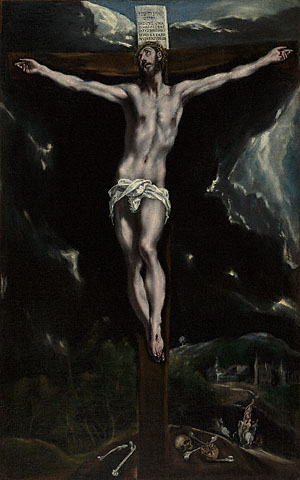
\includegraphics[width=0.9\textwidth]{elgreco.jpg}
   .\caption{Cristo crucificado de El Greco. Museo J. Paul Getty.} % URL: www.getty.edu/art/gettyguide/artObjectDetails?artobj=138292\&handle=li}
\end{figure}

\newpage

%Arte, estilo: Manierismo
%Cronología: Hacia 1600-1610
%Lugar: Museo J. Paul Getty, Los Ángeles
%Autor: El Greco
%Título: Cristo crucificado 

%Función: Purchased by a Spanish family at a flea market around 1950, it remained in their possession until recently. 
% http://www.ctv.es/USERS/ags/00013_mm.htm
% http://www.google.com/culturalinstitute/asset-viewer/christ-on-the-cross/cgHO8uo2dVOJoQ?hl=es&projectId=art-project


\begin{description}
\item[Estilo] Manierismo
\item[Cronología] Hacia 1600-1610
\item[Lugar] Museo J. Paul Getty, Los Ángeles
\item[Autor] Doménikos Theotokópoulos, más conocido como el Greco
\item[Título] Cristo crucificado
\end{description}

\textbf{Contexto histórico:}

El cuadro se realizó en plena contrarreforma. Durante este período la Iglesia católica intentaba consolidar su poder bajo la amenaza de la reforma protestante, es por eso que durante esta época se produjeron un gran número de obras de contenido religioso. De hecho la gran mayoría de las obras elaboradas por el Greco son de naturaleza religiosa, centrándose menos en retratos u otro estilo de obras. La obra a analizar es una de estas obras de carácter religioso.

En esta, y en general en todas sus obras, el Greco utilizaba un estilo propio basándose en el estilo veneciano en el uso del color y en el Manierismo alargando y retorciendo las formas y figuras. Dejó, de esta forma a un lado el orden, la claridad, la proporción y el equilibrio característico del Renacimiento anterior.

Se observan grandes contrastes en el uso del color en esta obra. Las figuras parecen emanar luz propia, pues están envueltas en oscuridad y exclusivamente hay luz en las formas que el autor quería que advirtiésemos. Además, esta utilización del color nos lleva a discernir la sombría situación del calvario de Cristo.

El alargamiento de las formas, propio de el Greco, provee a la obra de mayor belleza y misticismo, lo que le valió el reconocimiento de muchos religiosos de la época.

Siguiendo el estilo de su época el Greco representó la crucifixión de Cristo mediante tres clavos: un clavo que junta ambos pies a la cruz directamente y un clavo en cada palma de la mano, según la interpretación bíblica de la época, contrariamente a la creencia actual principal de que se encontraban a la altura de las muñecas.


\vspace{12pt}
\textbf{Anatomía de superficie:}

En esta obra el Greco nos muestra un Cristo que presenta una anatomía adecuada excepto en sus proporciones. La figura sigue una proporción de nueve cabezas, pudiendo apreciar, efectivamente la cabeza pequeña de la figura mientras el tronco y sus extremidades son extremadamente alargados, no concordando con ningún cánon de proporciones habitual \footnote{Actualmente existen tres cánones para determinar las proporciones de la figura humana: el cánon de siete cabezas y media, el cánon más relista en cuanto a medidas, que se considera la figura común, el cánon de ocho cabezas considerado la figura ideal y el cánon de ocho cabezas y media, con el que se representan las figuras heróicas.}. Sin embargo estas medidas dotan a la figura de una mayor heroicidad, presentando de esta forma, y junto con otros detalles de la obra, el triunfo de Cristo sobre la muerte, idea que en la contrarreforma querían destacar. Su longitud con los brazos extendidos es igual a su altura y el ángulo que forman entre ellos es de 135º.

Como la figura no ha fallecido no es posible observar las características típicas de la muerte como es la lividez del cuerpo o la laxitud muscular. Es más, la figura conserva los ojos abiertos, mostrando una ausencia de sufrimiento en el rostro, lo que es otro detalle de la obra en la que se ilustra el triunfo de Cristo, que inexpresivo mira al cielo (a Dios) a la espera de su muerte. La posición retorcida del cuerpo es utilizada por el autor para aumentar la belleza del cuadro, sin reparar en que es extremadamente difícil adquirir esa posición estando crucificado y al borde de la muerte. Tanto los músculos de los brazos como los de las piernas que contribuyen al mantenimiento de la postura están contraídos y extendidos, sin embargo los de la espalda, muy necesarios para el mantenimiento de esta postura no se observan claramente.

Apoya la mayor parte del peso del cuerpo sobre la pierna derecha aprovechando para inclinar la cadera hacia el mismo lado produciendo la curvatura del cuerpo de la que he hablado anteriormente y que se continuará en forma de \textit{S} a lo largo de la figura.

Además, existen otros signos que muestran el triunfo de la vida sobre la muerte. Uno de ellos es la escasa sangre que se visualiza en este cuadro, quitando de esta manera importancia a las heridas de la carne y dando una apariencia más divina. No encontramos la herida del costado derecho, lo que, de hecho, es lógico debido a que esta se le ocasiona después de morir, para verificar su muerte.

Para conseguir la postura que mantiene la figura intervienen varios músculos.
Tanto la espalda como el cuello se encuentran en posición erguida, con el rostro mirando hacia arriba, utilizando para ello los músculos erectores de la columna: los músculos del grupo iliocostal, los del grupo longuísimo y los del espinoso y los principales músculos del cuello como el esplenio y el esternocleidomastoideo, este último visible en la obra. Otro músculo que participa en la postura erecta es el recto del abdomen, el cual se puede discernir en la obra, junto con la línea alba, formada por la unión de vainas fibrosas en la línea media, y la línea semilunar, que marca el borde lateral del músculo recto del abdomen.

El músculo dorsal ancho que proviene de la espalda posee un tendón estrecho que envuelve al músculo redondo mayor formando el pliegue posterior de la axila, reconocible en esta imagen. Estos músculos producen la elevación del tronco estando los brazos fijos, por tanto tienen gran relevancia en la crucifixión. Además de estos dos músculos otro que participa en la elevación del tronco es el pectoral mayor que forma el pliegue anterior de la axila, también visible en la obra.

Otros músculos con gran relevancia en esta posición son: el trapecio, que se puede observar en la figura, y el elevador de la escápula, que elevan la escápula, y el serrato anterior que la gira. La posicion de Cristo en la cruz desplaza la escápula de esta forma.

El músculo deltoides se aprecia sin esfuerzo rodeando la articulación de los hombros en ambas extremidades superiores. Su principal función es la abducción del brazo y es por eso que se le confiere gran importancia en la posición en la que ambos brazos están en abducción.

En el brazo, aunque no con trazos muy firmes, son evidentes los músculos bíceps y tríceps. El primero se encuentra en la parte anterior del brazo y su principal función es la flexión de la articulación del codo, sin embargo en esta figura los brazos se encuentran en extensión por la que la función principal del bíceps no es la anteriormente citada sino la supinación del antebrazo, la cual la realiza junto con el músculo supinador. Por su parte el tríceps se encuentra en la parte posterior siendo su principal función la extensión de la articulación del codo, lo que posee importancia en esta posición. 

Las manos se encuentran en posición de reposo, por lo que el tercer, cuarto y quinto dedo se encuentran ligeramente flexionados, no siendo así, sin embargo, en el primer y el segundo dedo que se encuentran extendidos, posiblemente debidos a los clavos con los que se sujeta a la figura en la cruz. Estos no están representados en el centro de las palmas de las manos, como era habitual, si no que se sitúan entre los segundos y terceros huesos metacarpianos.

La caja torácica es fácilmente visible: el borde costal inferior, la depresión en la que se encuentra el esternón, algunas costillas (probablemente la tercera y la cuarta) e, incluso, ambas clavículas elevadas debido a la elevación de los brazos, que a su vez hace posible la óptima visualización de las estructuras anteriormente citadas. Igualmente, como el autor de la obra representa a un Cristo más bien delgado, la espina ilíaca puede ser divisada superficialmente en ambos lados de la pelvis.

La extremidad inferior izquierda mantiene la articulación de la rodilla ligeramente flexionada, mientras que la derecha la mantiene totalmente extendida. A su vez la cadera se encuentra ladeada hacia el lado de la pierna estirada, provocando que la espina ilíaca sea más fácilmente visible en este costado que en el izquierdo.
Los encargados de mantener esta postura son: en la extensión, el cuadriceps y los músculos del tracto iliotibial, y en la flexión, los músculos poplíteos y los gemelos. La rótula o patella, que se encuentra en la articulación de la rodilla se vislumbra perfectamente junto con la tuberosidad tibial en la rodilla flexionada. Aún así, la tuberosidad tibial, anatómicamente recta desde la articulación de la rodilla hasta la articulación del tobillo, se presenta curvada en el afán de el Greco por moldear las formas a su antojo

Los pies se encuentran uno sobre otro,el izquierdo sobre el derecho, y ambos clavados juntos en la cruz. Mantienen el peso de la mayor parte del cuerpo, ayudados por los músculos que elevan el tronco y los clavos que sujetan ambos brazos.
\section{Análisis de la obra pictórica: Cristo crucificado de Velázquez } 

Arte, estilo: Barroco

Cronología: 1632

Lugar: Museo del Prado, Madrid,España

Autor: Diego Velázquez

Título: Cristo crucificado

Función: Aunque se encontraba en el Convento de la encarnación de San Plácido, no está claro donde estuvo los primeros años tras su realización ni la función específica que desarrollaba. Posteriormente se tiene constancia de que estuvo en la sacristía de este convento hasta alrededor del 1804, año en el que Godoy lo compra al convento. Pasa después por distintas manos, llegando finalmente al Museo de Prado en 1829, donde permanece actualmente. % El Cristo crucificado de velazquez, trasfondo histórico religioso. % http://www.museodelprado.es/coleccion/galeria-on-line/galeria-on-line/obra/cristo-crucificado-1/

\textbf{Anatomía de superficie}
En esta obra Velázquez nos cautiva con una figura con una postura serena y de proporciones y anatomía estudiadas. Responde a un modelo de siete cabezas y media. Su longitud con los brazos extendidos es igual a su altura y el ángulo que forman entre ellos es de 113º. La cadera esta ligeramente inclinada hacia el lado derecho, dando la sensación de apoyo del peso en el lado izquierdo, lo que se podría interpretar como un ligerísimo contrapposto clásico.
En el cuadro se puede observar la parte izquierda de la cara, la parte derecha está cubierta por el cabello que cae sobre ella. En cuanto a aquello que podemos ver, se trata de una cara inexpresiva con barba que cubre parte de las mejillas y el mentón. Bajo esta barba se puede apreciar la forma del hueso de la manbíbula (cuerpo, rama y ángulo). La mucosa de los labios es apenas visible entre el vello, aunque sí se intuyen incluso la comisura labial izquierda. La nariz se presenta en el centro de la cara de forma piramidal. La estructura de la nariz la proporcionan los huesos nasales que articulan entre sí, con el hueso frontal(por donde se une a la frente) y con el hueso maxilar (por el que se une  a las mejillas). La parte más prominente de la nariz es el cartílago nasal que separa las dos fosas nasales. Se aprecia el espacio del surco naso-labial, aunque éste no se ve directamente, porque al igual que el mentón, está cubierto de vello. Sin embargo, sí se distingue la aleta nasal izquierda y el septo nasal, a la vez que se puede intuir la narina izquierda de la nariz. Se puede también vislumbrar una pequeña arruga, la línea naso-labial. Se puede ver la prominencia de la mejilla, formada por el hueso cigomático. Entre la nariz y la frente se encuentra una depresión denominada nasión. La frente, formada por la convexidad lisa del hueso frontal, apenas es visible puesto que está tapada por la corona de espinas. Sus bordes inferiores (arcos supraciliares) dan lugar al borde superior de cada órbita. Además estos dos arcos se unen mediante un puente denomindo gabela. Superficialmente a estas elevaciones se encuentran las cejas. Medialmente el globo ocular está limitado por los huesos maxilar y frontal que articulan entre ellos, lateralmente está limitado por los huesos frontal y cigomático e inferiormente por el hueso maxilar. El globo ocular izquierdo no es visible, solo se adivina debajo del párpado superior que lo cubre, en el que además se puede observar una pequeña arruga. Sí se puede vislumbrar las uniones medial y lateral entre los párpados superior e inferior, que limitarían la hendidura palpebral en caso de estar abiertos. En sus bordes se encuentran las pestañas, manifestadas en la obra mediante una línea más oscura en el borde de los párpados. Ambas orejas están tapadas por el cabello, por lo que sus partes no son visibles.
El resto de la cabeza está formada por la bóveda craneal, la cual se insinua debajo del cabello. La cara lateral de la bóveda la componen los huesos frontal, parietal, occipital y temporal.
El cuello no es visible, al estar la cabeza caída hacia abajo, ésta tapa las estructuras anatómicas del cuello.

En la imagen se puede observar el torso desnudo de Cristo crucificado, en el que se aprecian una serie de estructuras anatómicas. 

Al tratarse de un individuo delgado se puede intuir la caja torácico perfectamente. Vislumbramos, a duras penas, la clavícula izquierda que articula con el esternón (manubrio) y la primera costilla, la derecha, no es visible, puesto que está tapada por el cabello. El borde costal inferior formado por las seis últimas costillas es fácilmente visible, al igual que la depresión en la que se encuentra el cuerpo del esternón y el contorno de algunas costillas (probablemente la cuarta, quinta, sexta y séptima), sobre todo las del lado derecho, ya que la sombra del propio cuadro nos  impide ver bien las del izquierdo. La escotadura esternal, también se puede intuir sobre la cara superior del manubrio, sin embargo, hay que dejarse llevar un poco por la imaginación, ya que, de nuevo la sombra del cuadro nos impide su correcta visualización. No se observa la apófisis xifoides, que está cubierta, por el recto anterior del abdomen, lo que se considera normal.

En cuanto a los músculos podemos vislumbrar el pectoral mayor, que inserta en el borde interno de la clavícula, en los cartílagos de las seis costillas superiores y en el húmero, formando así el pliegue anterior de la axila, muy claro en la imagen, junto con el músculo deltoides, que se puede contemplar recubriendo la articulación del hombro. Lateralmente no se observan claramente los músculos. El serrato anterior que inserta en el borde anterior interno de la escápula, y en las ocho costillas superiores, junto con sus interdigitaciones con el músculo oblicuo externo podrían ser visibles en un individuo delgado y musculoso como el Cristo que representa este cuadro, sin embargo no es fácil de reconocer. Sí se puede apreciar el músculo dorsal ancho, proveniente de la espalda e insertado en el ángulo inferior de la escápula. Su tendón estrecho envuelve al músculo redondo mayor que forma el pliegue posterior de la axila. Este va desde el borde lateral de la escápula hasta el surco bicipital del húmero. El borde lateral de la escápula puede percibirse a través de la masa del redondo mayor.
Los pezones se encuentran en el Cristo de la obra alrededor del cuarto espacio intercostal, lo que es anatómicamente correcto.

En el abdomen, que delimita superiormente con el reborde costal, que como ya he dicho es claramente visible en esta obra, se encuentran los músculos abdominales, que se pueden apreciar, aunque no muy marcados. Estos músculos forman una vaina fibrosa a cada lado de la línea media que se unen en esta, formando la línea alba. La figura no está suficientemente musculada para poder apreciar las tres inserciones tendinosas que se encontrarían encima del ombligo, a duras penas podríamos localizar una de ellas. Sí se divisa bastante bien la línea semilunar, que marca el borde lateral del músculo recto del abdomen. La espina ilíaca si se aprecia, sobre todo en el lado derecho, que es el lado hacia el que está ligeramente inclinada la cadera.
El músculo mas superficial de los músculos laminares del abdomen es el oblicuo externo , pero como ya he comentado anteriormente no se ve claramente, y aunque sepamos que tiene que estar ahí, sus interdigitaciones con el serrato anerior no son visibles en el cuadro. Este músculo se inserta superiormente en las ocho costillas inferiores e inferiormente en la sínfisis de púbis, tuberosidad púbica, espina ilíaca anterosuperior y cresta ilíaca. Entre la espina y la tuberosidad púbica gira sobre sí mismo y forma el ligamento inguinal. La depresión que suele haber a la altura de ese ligamento, y que suele ser más visible en hombre, se puede observar perfectamente en la obra pictórica.
Las estructuras pélvicas no son visibles, debido a que el autor coloca encima un paño blanco con el que las tapa.

Las extemidades superiores se encuentran extendidas cada una hacia un costado de la cruz: Los músculos son visibles claramente. Antes de empezar con los músculos del brazo propiamente dichos, remarcaré algúno que se encuentra sustentando la articulación del hombro. El múculo trapecio sí se observa, este lateralmente se inserta en el tercio externo de la clavícula, el acromion y la espina de la escápula. Estas estructuras no son visibles anteriormente en la posición en la que se encuentra la figura analizada (brazos extendidos hacia los lados), sin embardo podemos apreciar un hueco en la unión de este músculo a las estructuras previamente citadas. El músculo que no nos deja ver esas estructuras es el deltoides, que también se ve fácilmente redondeando la articulación del hombro por su parte superior, cubriendo la epífisis proximal del húmero. Se inserta medialmente, al igual que el trapecio, en la clavícula, el acromion y la espina de la escápula y lateralmente en el tubérculo deltoideo de la cara lateral del húmero. Es el principal abductor del brazo por lo que tiene gran relevancia en esta posición.
En el brazo se observan tanto el bíceps como el tríceps. El bíceps forma una prominencia en la parte anterior del brazo. Tiene dos cabezas, de las cuales la corta inserta en la apófisis coracoides y la larga en la cara superior de la fosa glenoidea de la escápula. Distalmente se inserta en la tuberosidad bicipital del radio, pasando por el medio de la fosa cubital.
En ambos brazos podemos distinguir la fosa cubital. Esta está limitada superiormete por la línea que va desde la epitróclea hasta el epicóndilo del húmero, lateralmente por el músculo braquiorradial y medialmente por el pronador redondo.
Los huesos de la articulación del codo suelen ser evidentes. En esta obra no se pueden distinguir claramente las distintas estructuras debido a la posición de los brazos (se verían mejor desde la cara posterior). Lo único que se aprecia de forma clara es la epitróclea del húmero.
Los brazos se encuentran en total supinación y extensión. La extensión la realiza el tríceps junto con la contribución de los músculos del origen del extensor común. Y de la supinación se encargan el bíceps y el supinador.

A la altura de las muñecas podemos observar las apófisis estiloides del cúbito y del radio, que en una persona un poco más gruesa no serían visibles. Además, se podrían intuir los tendones de los músculos del antebrazo que pasan a la mano. Cuando se flexiona la muñeca sobresalen tres tendones. El flexor carpi raialis se inserta distalmente en la base de los metacarpos 2 y 3, el flexor carpi ulnaris de inserta en el pisiforme y de allí en el ganchoso y en la base del quinto metacarpiano.
Las venas, tanto cefálica como basílica suelen se visibles en mayor o menor medida en hombres jóvenes, delgados y en cierta medida musculados, no obstante, no han sido dibujadas por el artista en esta figura.
En la obra se puede apreciar la palma de la mano derecha, aunque parcialmente, pues en ella se encuentra clavado el clavo a la cruz y, además los dedos se encuentran ligeramente flexionados, por lo que podemos vislumbrar las articulaciones interfalángicas en ellos. El metacarpiano del primer dedo también lo podemos distinguir en el cuadro. Este posee más movilidad que el resto de los metacarpianos, que además no son visibles en el cuadro, puesto que están tapados por los músculos de la palma.
En la mano izquierda básicamente se observan las mismas estructuras que en la derecha. Pero además podemos percibir la denominada tabaquera anatómica. La tabaquera anatómica es una concavidad presente en la cara lateral de la muñeca, que se evidencia más al extender el primer dedo. Está limitada por varios tendones: el abductor largo del pulgar, que se inserta distal al primer metacarpiano; el extensor corto del pulgar, que se inserta en la falange proximal del pulgar; y el extensor largo del pulgar, que inserta en la falange distal del primer dedo.
En las palmas de ambas manos se observan tanto la eminencia tenar, como la hipotenar.
La emnencia tenar se denomina al abultamiento lateral presente en la palma de la mano, a la altura del primer dedo. Está formada por los músculos cortos del pulgar: los músculos abductor, flexor y oponente del pulgar.
La eminencia hipotenar se denomina al abultamiento medial de la palma de la mano a la altura del quinto metecarpiano. Está formada por el abductor, el flexor y el oponente del meñique.
Podemos apreciar cierta flexión en las articulaciones metacarpofalángicas, la cual es producida por los músculos lumbricales que se encuentran entre los dedos. Los dedos también mantienen cierta flexión, producida esta por los tendones de los flexores superficial y profundo de los dedos.
\subsubsection{Visión anterior del antebrazo}
El músculo pronador se inserta sobre la cara anterior de la epitróclea y en la región central del radio. Es un pronador del antebrazo. Los tendones de los músculos flexor carpi radialis, palmar mayor, flexor superficial de los dedos y flexor carpi ulnaris pasan a la mano. Son también flexores débiles del codo.
El músculo braquiorradial se inserta proximalmente  en los dos tercios superiores de la cresta supracondílea del húmero y distalmete en la cara lateral de la epífisis distal del radio. Este músculo prona o supina el antebrazo.

El pisiforme es visible, así como el tubérculo del escafoides.

Podemos apreciar claramente la masa muscular de las estremidades inferiores, ya que estas se encuentran al descubierto. Sin embargo no es así de fácil distinguir los músculos específicos que producen esta masa muscular.
Podemos intuir a duras penas por donde pasa el músculo sartorio, que que inserta en la espina ilíaca y en la superficie subcutánea medial de la parte superior de la tibia. Así mismo se podría señalar el músculo cuadriceps, músculo principal de la cara anterior del muslo, junto con sus tres cabezas superficiales: vasto externo, vasto interno y recto anterior, no el vasto intermedio, que va bajo el recto anterior. Los músculos pectíneo, psoas-ilíaco y recto interno no son visibles pues están tapados por el paño blanco que también tapa las estructuras pélvicas. No son claramente apreciables otros músculos superficiales como el tensor de la fascia lata (que inserta en la cara externa del ilion y en la tibia, formando el tracto iliotibial al unirse con el glúteo mayor), que esta situado en el lateral del muslo, superficialmente al trocánter mayor del fémur.
El músculo cuadriceps forma en su parte inferior el "ligamento patelar" que recubre la rótula y se inserta en la tuberosidad tibial. En una figura delgada como esta la rótula o patella se puede apreciar, al igual que la tuberosidad tibial, aunque son más fáciles de apreciar en la flexión de la rodilla.
El resto de estructuras de la rodilla no son apreciables, aunque se pueden intuir: condilos femorales, ligamentos de la articulación, tubérculo adductor del fémur, retináculos rotulianos medial y lateral...
Las articulaciones de las rodillas de la figura se encuentran una en posición de extensión,mientras que la ptra se encuentra ligeramente flexionada. Los músculos encargados de la extensión son: el cuadriceps y los músculos del tracto iliotibial, y los de la flexión son: los músculos poplíteos y los gemelos.
Podemos apreciar la tibia desde latuberosidad tibial hasta el maleolo medial, en su recorrido subcutáneo.
La masa muscular que se puede visualizar la conforman varios músculos. El músculo tibial anterior se encuentra en el lateral de la pierna y es el único de los cuatro músculos que inserta en la tibia. Además tiene un tendón distal que pasa hacia la base del primer metatarsiano. Otros músculos que forman esta masa muscular son el extensor largo del dedo gordo y el extensor largo de los dedos. Sin embargo también se pueden apreciar en la cara lateral músculos que en principio forman parte de la parte posterior: el sóleo y una de las cabezas del gemelo (superior al sóleo), que se unen para formar el comunmente denominado tendón de aquiles. Más lateral se encuentra el músculo peroneus tertius.
A la altura de la articulación del tobillo se pueden contemplar ambos maleolos, interno formado por la tibia y externo formado por el peroné (que en el resto de su recorrido por la pierna está rodeado por músculos). Anatómicamente el maleolo externo se encuentra un centímetro más abajo que el maleolo interno. En la representación pictórica se reproduce correctamente esta característica.

Al estar de pie sobre una pierna el lado de la pelvis que no soporta peso se eleva para evitar que la pierna libre no pise el suelo. Esta acción está realizada por los glúteos medio y menor.

Los pies se encuentran apoyados en una tabla,lo que permite que sus rodillas y cadera estén ligeramente flexionadas. Apoyados sobre el hueso calcáneo y la articulación metatarsofalángica, cuya prominencia es visible bajo la grasa subcutánea que sirve de almohadilla, dejan intuir claramente el arco plantar, mantenido por los músculos cortos y los tendones del flexor largo. Los pies se ubican en paralelo entre ellos ligeramente suparados aneriormente, con un clavo en cada dorso y sangre que emana de la herida, lo que nos hace más dificil la visión de las estructuras que se encuentran en el dorso del pie. La cara lateral es peor visible, debido a la gran dfuminación de los colores en esta zona y a la oscuridad con la que el artista simula la sombra de la figura. Más medialmente se pueden observar tendones (del músculo extensor largo de los dedos, del músculo extensor largo del dedo gordo y de los músculos peroneos) y prominencias óseas que no son claramente distinguibles. En la parte anterior, los dedos se encuentran relajados y las uñas nacen de cada uno de ellos superficialmente.
El extensor corto de los dedos es el único músculo situado en el dorso del pie y se extiende desde el hueso calcáneo. Sus tendones se insertan en la falange proximal del primer dedo y en la cara lateral de los tendones del extensor de los dedos segundo, tercero y cuarto.

La cara posteromedial del calcáneo, el sustentaculum tali, el tubérculo del navicular.


Colores: primarios, secundarios, fríos, cálidos, paleta de colores.

Línea, dibujo

Luz

Perspectiva

Movimiento o quietud

Proporciones

Iconografía

Resolución del tema

Momento de la narración elegido

\section{Análisis de la obra pictórica: Cristo amarillo de Gauguin}

Arte, estilo: Fauvismo

Cronología: 1889

Lugar: Albright-Knox Art Gallery, Buffalo, Estados Unidos

Autor: Paul Gauguin

Título: El Cristo amarillo (Le Christ jaune)

Función: 
\section{Análisis de la obra pictórica: Cristo de San Juan de la Cruz de Dalí}

\begin{figure}[ht!]
    \centering
    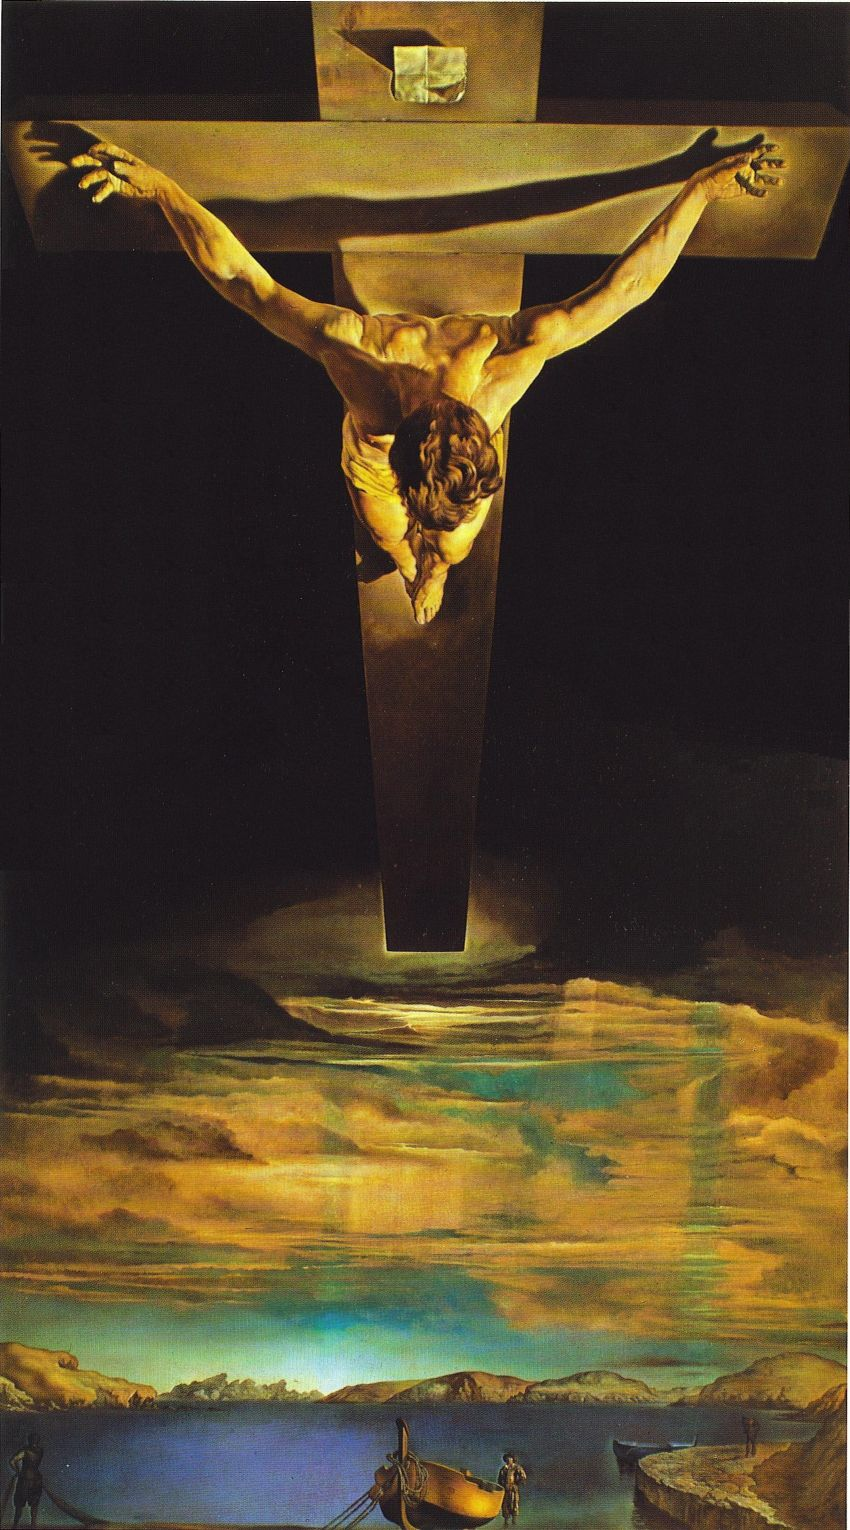
\includegraphics[width=0.84\textwidth]{dali.jpg}
   .\caption{Cristo de San Juan de la Cruz de Salvador Dalí. Museo Kelvingrove.} % URL: blogsantiagosoul.wordpress.com/tag/viva-la-vida}
\end{figure}

\newpage

%Arte, estilo: Surrealismo
%Cronología: 1951
%Lugar: Museo Kelvingrove, Glasgow, Reino Unido
%Autor: Salvador Dalí
%Título: Cristo de San Juan de la Cruz

%Función: Se expuso por primera vez en la galería Lefevre de Londres. %http://www.xn--esarteespaol-jhb.es/contenido.php?recordID=11

\begin{description}
\item[Estilo] Surrealismo
\item[Cronología] 1951
\item[Lugar] Museo Kelvingrove, Glasgow
\item[Autor] Salvador Dalí
\item[Título] Cristo de San Juan de la Cruz
\end{description}

\textbf{Contexto histórico:}

Esta obra se realizó en plena dictadura franquista, en la que numerosos artistas fueron desterrados por no compartir las ideas de la dictadura. No siendo así para Dalí que no sólo aceptó la dictadura franquista, sino que incluso elaboró un retrato de la nieta del propio Franco.

Gran pintor de estilo surrealista, Dalí siguió un estilo propio y más extravagante que el del resto de sus compañeros. El surrealismo nació en 1924, en París a manos de André Breton que publicó el \textit{Primer Manifiesto Surrealista}. Los pintores de esta corriente, influidos enormemente por las teorías de Freud, intentaron expresar en sus obras el mundo del subconsciente.

Dalí enseguida sobresalió en este estilo con una primera etapa más agresiva. Sin embargo, a partir del 1948, cuando regresó a Europa de América, inició una etapa en la que vuelve al clasicismo, reproduciendo sus primeros temas religiosos. Una de estas obras religiosas es la del Cristo de San Juan de la Cruz. Este Cristo está basado, como su nombre indica, en el Cristo dibujado por San Juan de la Cruz tras una revelación.

Dalí decidió representar \textit{un Cristo bello como el mismo Dios que él encarna} y no centrase en la fealdad para provocar la emoción en el espectador. Lo hizo adoptando una perspectiva totalmente nueva de la crucifixión. Con este nuevo enfoque situó a Cristo en la Cruz en una posición vertical y casi perpendicular al espectador de la obra.

Además decidió retirar todos aquellos elementos que intervinieron en la crucifixión de Cristo, nótese que éste no conserva la corona de espinas ni ninguna herida, tampoco están dibujados los clavos que lo deberían sostener en la cruz, en la que parece que está suspendido por arte de magia.

Debajo de la imagen principal del cuadro se puede apreciar un paisaje, supuestamente representado a partir de la bahía de Port Lligat. En ella se ven dos pescadores que, sin embargo, están inspirados en los pintores Le Nain y Velazquez.

El Cristo se sitúa en un fondo oscuro que le da una imagen dramática a la obra junto al contraste con la iluminación que se proyecta en forma de rayo de luz sobre la figura. Entre la imagen del crucificado y la de los pescadores se interpone un cielo nuboso, que aporta a la obra aún mayor dramatismo al separar la crucifixión y la imagen de la tranquila bahía de pescadores, dando a entender la indiferencia de éstos ante el suceso que se está produciendo.

% http://www.artehistoria.jcyl.es/v2/obras/9639.htm
% http://unapizcadecmha.blogspot.com.es/2013/11/el-cristo-de-san-juan-de-la-cruz-1951.html
% http://www.arteespana.com/salvadordali.htm
% Artículo de San Juan de la Cruz
% libro de aita

\vspace{12pt}
\textbf{Anatomía de superficie:}

En esta obra en la que Dalí refleja una nueva perspectiva de la crucifixión de Cristo, siendo la cabeza de éste el centro de la obra, podemos observar un Cristo de con características totalmente diferentes a las apreciadas en la mayoría de obras acerca de la crucifixión. Aparte de tener el pelo corto, al contrario que en las numerosas obras en las que se representa a Cristo, no posee signos de sufrimiento, ni clavos que le sujeten a la cruz, ni corona de espinas, ni tampoco sangre puesto que no hay heridas de las que pueda brotar.

Aún sin elementos de crucifixión la figura mantiene una posición en la que se sugiere que ambos pies estarían unidos a la cruz mediante el mismo clavo, mientras que los clavos de las extremidades superiores se encontrarían en las palmas de las manos. Esto último se puede percibir en la caída del cuerpo hacia delante que ocurre desde más arriba de las muñecas, según la sombra que se proyecta detrás.

Al estar la cabeza inclinada hacia delante, no es posible ver el resto del cuerpo de la figura, sin embargo si ofrece una visión espectacular de la espalda y de sus músculos. Los brazos caen extendidos, formando un triángulo con la cruz que mantiene suspendido a Crsito y dando una sensación de que éste se encuentra colgado boca abajo por el espacio que hay entre su cuerpo y la cruz.

El autor en esta obra de arte no se centra en el sufrimiento y la muerte de Cristo, sino que intenta evocar la belleza de Cristo Dios. Por ello se puede considerar admirable la simetría del cuerpo y la anatomía que se vislumbra. La actitud de la figura es relajada, pudiéndose observar este hecho en la posición de sus brazos y de los músculos de la espalda.

No es posible saber si el Cristo se encuentra fellecido o al borde de serlo en la obra, puesto que el autor ilumina la figura con una luz amarillenta que crea un gran contraste entre las zonas iluminadas y las zonas en sombra y no deja observar el verdadero color del cuerpo de la figura.

Diferentes estructuras anatómicas se pueden observar en esta obra de acuerdo a la perspectiva y posición de la figura, que no coinciden con las descritas en figuras anteriores.

Los músculos de la espalda y los de la parte posterior del cuello, aunque totalmente relajados, son claramente visibles. Sin embargo el claroscuro utilizado por el autor dificulta la identificación de estos.

La línea del ligamento nucal que recorre las vertebras cervicales si se observa, no identificando de manera correcta las apófisis espinosas de las vertebras cervicales inferiores, especialmente la de la C7, que por la postura tendrían que ser fácilmente visibles. 

La masa muscular del cuello la componen el músculo esplenio, el músculo esternocleidomastoideo y el trapecio, que se inserta superiormente en la línea nucal superior y también ocupa gran espacio de la espalda.

En la espalda, cubiertas por el músculo trapecio, se perciben las siluetas de las escápulas. Éste músculo junto con  el serrato anterior, que no es visible en la figura, realiza la rotación externa de las escápulas, necesaria en la posición adoptada por la figura de la obra.

En la masa muscular de los brazos se aprecian los deltoides que son los principales músculos abductores del brazo, recubriendo el hombro. Además de extendido el brazo está en posición de supinación. De la extensión se encarga el tríceps braquial, mientras que la supinación requiere de la acción del músculo braquiorradial, que se encuentra en el antebrazo. Las manos se encuentran en posición de descanso, apreciando cierta flexión de las articulaciones interfalángicas y metacarpofalángicas provocada por los músculos flexor carpi radialis, palmar mayor, flexor superficial de los dedos y flexor carpi ulnaris que pasan del antebrazo a la mano.

Anteriormente se aprecia el músculo pectoral mayor que forma el pliegue anterior de la axila. Sin embargo ésta no se ve, puesto que queda tapada por el hombro y su propio pliegue anterior.

El tórax, abdomen, pelvis y parte de la extremidades inferiores están ocultas por la cabeza, que cae hacia delante. únicamente podemos apreciar parte del muslo, las articulaciones de las rodillas y los pies, diminutos debidos a la perspectiva. La principal masa muscular del muslo es el cuadriceps, cuya función es la extensión de la rodilla, el borde lateral del muslo lo forma el músculo sartorio, el cual nos permite cruzar las piernas. Ambos movimientos imprecindibles para la postura de Cristo con ambas piernas extendidas y crucificado con un pie encima del otro.

Sin embargo, la articulación de la rodilla de la pierna izquierda, está ligeramente flexionada para permitir que el pie de esta extremidad pueda situarse encima del pie de la extremidad derecha. La flexión de la rodilla está realizada por varios músculos: los isquiotibiales, el sartorio, el poplíteo y los gemelos.

\section{Resultados y discusión}
\section{Conclusión}
Tras haber realizado el análisis de varias obras de distintas épocas se pueden sacar varias ideas en claro.

Las obras se rigen por el estilo predominante de la época, aunque en ocasiones los autores de éstas aporten novedades en el arte de su tiempo, como Mantegna que revolucionó la perspectiva con su lamentación sobre Cristo muerto o Dalí con su estilo único.

La intención del autor también cambia. Algunos autores intentan mostrar una obra bella utilizando para ello proporciones y armonía, como Velázquez o Dalí, mientras que otros utilizan la prevalencia del realismo para crear una obra que represente la muerte de Cristo de una forma lo más exacta posible a la realidad, éste es el caso de Mantegna o Miñarro.

En relación a la anatomía, %se ve diferencia entre aquellas obras anteriores a las disecciones del cuerpo y aquellas en las que el conocimiento del cuerpo era mayor.
la figura de la obra de Mantegna posee una anatomía estudiada, sin embargo no es en lo que más se centra, numerosos detalles en la obra son más impresionantes, como la perspectiva que adopta la figura de Cristo o los rasgos referentes a la muerte que éste presenta. Velázquez sí que se centra mucho en la anatomía superficial y en las proporciones del Cristo de su obra. Dalí, por su parte, se propone dibujar el Cristo más bello, para el que adopta una perspectiva nueva e incluso se dice que utiliza un modelo para representar de forma correcta la anatomía. Miñarro, por su parte, se basa en la Síndone de Turín para intentar representar la muerte de Cristo como nunca hasta ahora se había visto, en toda su crudeza.

%El número de clavos con el que Cristo aparece clavado en la Cruz es variable debido, más a las ideas del propio autor que a las de la época. De hecho, en todas las obras analizadas se puede observar la inserción de tres clavos, uno uniendo los dos pies y otro en cada extremidad superior, excepto en la obra de Velázquez que se deja influir por su maestro, y no así por su tiempo. Otro detalle sobre la inserción de los clavos es que a lo largo del tiempo el Evangelio de San Juan ha sido interpretado de forma que incluso en épocas más modernas estos se han seguido representado en la palma de la mano y no ha sido hasta hace varias décadas que se han hecho experimentos en cuanto a ello. Por ello, en la obra de Miñarro es en la única que se pueden apreciar los clavos a la altura de los carpos y no entre los metacarpos como se representa en las demás obras.

En cuanto a la representación de la muerte de Cristo, Mantegna en su obra presenta la laxitud en la postura y la rigidez en algunos músculos, que probablemente está relacionada con el \textit{rigor mortis}, además de la lividez con la que el autor ilustra el cuerpo, reproduciendo de manera bastante acertada la apariencia de un cadáver.

Velázquez, sin embargo, realiza una obra en la que no reproduce la muerte de Cristo. El Cristo no posee ninguna característica de un cuerpo muerto, ni laxitud en los músculos ni lividez cadavérica. Es más, muestra ciertas características que nos llevan a la conclusión de que el Cristo no ha fallecido e icluso se encuentra en relativas buenas condiciones, sobre todo, tratándose de una figura que ha soportado toda clase de martirios.

Dalí propone la imagen de un Cristo que no porta nungún elemento utilizado para su suplicio ni crucifixión. Aún así, nos muestra una cristo cuyos músculos están relajados, como si estuviese a punto de fallecer o ya hubiera fallecido. En cuanto a la coloración del cuerpo, es dificil de determinar si posee el característico del \textit{livor mortis} o no, debido al gran contraste de luz que Dalí utiliza en la obra.

En el Cristo de la Síndone de Miñarro se distinguen fácilmente las características de la muerte en la figura. De hecho ésta posee un \textit{rigor mortis} con una rigidez muy marcada y un \textit{livor mortis} que se aprecia en el color ceniciento del cuerpo, así como en el acúmulo de sangre en la zona más distal de las extremidades inferiores.
\newpage
\begin{appendices}
\section{Resumen del libro: Anatomía de superficie: las bases anatómicas del examen físico}

\subsection{CABEZA}

\subsubsection{Cara}

\paragraph{Huesos de la cara:} La frente esta formada por la convexidad lisa del hueso frontal. Sus bordes inferiores (arcos supraciliares) dan lugar al borde superior de cada órbita.Estos dos arcos se unen con un puente denominado gabela. La depresión que hay debajo (entre la frente y la nariz) es el nasión.
El hueso maxilar articula con el frontal formando la cara interna de la órbita y junto con el hueso lacrimal aloja al aparato lacrimal.
La nariz  está formada por los huesos nasales que articulan entre sí y con los huesos frontal (por arriba) y maxilar (por el lado). Las suturas internasales y frontonasales se cruzan en el nasión.Además la parte más promiinente de la nariz esta formada por el cartílago nasal que separa las fosos nasales con el septo nasal
El borde externo de la órbita está formado por los huesos frontal y cigomático. Este último forma también la prominencia de la mejilla y el arco cigomático (junto con la apófisis cigomática del hueso temporal)y junto con el hueso maxilar el borde inferior de la órbita.
El borde inferior del maxilar presenta los alveolos para los dientes superiores, así como el hueso de la mandíbula contiene los de los huesos inferiores.

\paragraph{Músculos de la cara:} Los músculos de la cara contribuyen mayoritariamente a dotar a la cara de expresión facial. Estos músculos se disponen como esfínteres (músculo orbicular del ojo y músculo orbicular de la boca) y dilatadores alrededor de la órbita, nariz y boca. Además existe el músculo frontal que se une con la apófisis occipital y la platisma que se une al tejido subcutáneo del cuello y del toráx superior.

El resto de la cabeza está formada por la bóveda craneal. La cara lateral de la bóveda la componen los huesos frontal parietal occipital y temporal.
Las apófisis de los huesos frontal y cigomático (que forman el borde externo de la órbita)forman el borde anterior de la fosa temporal. La línea temporal da inserción a la fascia del músculo temporal  (puede sentirse al masticar)que inferiormente se inserta en el arco cigomático.
El músculo masetero va desde la cara externa posteroinferior de la mandíbula al borde inferior del arco cigomático (se acentúa al apretar los dientes).
Detrás de la oreja se encuentra la apófisis mastoides (recubierta por el esternocleidomasoideo y el músculo digástrico).

\subsubsection{Mandíbula}
Cuerpo, rama y ángulo. El cóndilo mandibular se palpa con dificultad con la mandíbula cerrada pues está cubierto por el ligamento lateral, pero se hace visible al abrir la mandíbula.

\subsubsection{Órbita - globo ocular}
Limitada anteriormente por los párpados superior e inferior que estań unidos en sus extremos medial y lateral, limitando la hendidura palpebral. En sus bordes se encuentran las pestañas dispuestas en dos o tres hileras irregulares. En el lado medial se encuentra la carúncula lacrimal, que se une al saco lacrimal mediante los canalículos lacrimales (no visibles). Los párpados estan rodeados por el músculo orbicular y el superior se eleva por la acción del músculo elevador del párpado. Los movimientos oculares se deben a los músculos extraoculares.

\subsubsection{Cavidad oral}
Es el principio del tubo digestivo y su membrana mucosa comienza en la cara anterior de los labios (parte rosada). Contiene lengua, las arcadas dentarias con encías y dientesy recibe los orificios de salida de las glándulas salivares. Existen el paladar duro, formado por los huesos maxilar y palatino y el paladar blando que termina en la úvula. La lengua descanas sobre el suelo de la boca. El frenillo une la cara inferior de la lengua con el suelo de la boca.

\subsubsection{Oreja}
Formada por piezas de fibrocartilago dispuestas de forma irregular a las que se une la piel. Hélix, antihélix, trago, antitrago, lóbulo, orificio auditivo externo.


\subsection{CUELLO}

\subsubsection{Visión anterior}
Delimitado superiomente por la mandíbula (cuerpo y ángulos), inferiormente por la hendidura esternal del manubrio y las clavículas. Las clavículas articulan con el esternón (unión esternoclavicular) y con el acromion (unión acromioclavicular).
El músculo esternocleidomastoideo se inserta en la apófisis mastoides y tercio externo de la línea nucal superior por su límite superior y en el esternón y la clavícula por su parte inferior. Los bordes anteriores de la parte esternal y de la parte clavicular forman una V prominente cuando se contraen simultáneamente (cuando se eleva la cabeza en posición de decúbito supino).

Laringe: Se sitúa en la línea media del cuello. Puede verse cómo se eleva durante la deglución. En el borde superior se encuentra el hueso hioides (forma de U) a nivel de la cuarta vértebra cervical. El cartílago tiroides forma una prominencia en la línea media que es más evidente en el varón (angulo entre sus alas 90º, mientras en la mujer 120º). Las cuerdas vocales se insertan en su parte posterior y los músculos se unen al hueso con el hioides superiormente y al dorso del manubrio inferiormente. El cricoides forma parte del borde inferior de la laringe y es el único anillo completo de cartílago en la vía respiratoria (los demás están incompletos por su cara posterior). La glándula tiroides está formada por varios lóbulos y un itsmo que los une (línea media anterior al segundo o tercer cartílagos traqueales). La glándula no se aprecia, sin embargo si aumenta de tamaño (bocio) se puede ver cómo se mueve con la laringe. 

Región submandibular: El triángulo anterior (esternocleidomastoideo, rama mandibular y línea media) contiene otros tres triángulos formados por dos músculos insertados en el hueso hioides. El triángulo digástrico formado por el vientre anterior y posterior del músculo digástrico (unidos por un tendón al hueso hioides) y el borde inferior de la mandíbula. El triángulo carotídeo formado por el vientre posterior del músculo digástrico, el músculo omohioideo y el esternocleidomastoideo. Y el triángulo muscular delimitado por el omohioideo, el vientre anterior del digástrico y la línea media. El triángulo digástrico contiene la glándula submandibular que descansa sobre y alrededor del borde posterior del músculo milohioideo (de la lengua al hioides). 

\subsubsection{Visión lateral}
Delimitado superiormente por cuerpo, ángulo y ramas de la mandíbula y la articulación temporomandibular Inferiormente está delimitada por la clavícula y el acromion que forman el vértice del hombro (articulación acromioclavicular).
El triángulo posterior formado por esternocleidomastoideo, clavícula y músculo trapecio. En un individuo delgado con la cabeza vuelta y flexionada al lado contralateral se pueden ver el omohioideo cruzando el triángulo y el músculo escaleno anterior descendiendo.

\subsubsection{Visión posterior}
Delimitada superiormente por la línea nucal superior del hueso occipital que termina medialmente en la protuberancia occipital externa y lateralmente en la apófisis mastoides.
El ligamento nucal se encuentra en la línea media y se inserta en el hueso occipital y en las apófisis espinosas de las vértebras cervicales. Son visibles las apófisis espinosas de las dos o tres vertebras cervicales inferiores, así como todas las torácicas. La apófisis espinosa de la séptima vertebra cervical  y la primera torácica son las más evidentes. También son visibles, el acromion y la espina escapular.
El músculo trapecio se inserta superiormente en el tercio medio de la línea nucal superior.


\subsection{TÓRAX}

\subsubsection{Pared torácica anterior}
Desde las clavículas hasta el borde costal inferior. Formado por el esternón, las costillas y cartílagos costales y los músculos relacionados.
El esternón está formado por tres partes: el manubrio, el cuerpo y la apófisis xifoides. Se puede observar la escotadura external sobre la cara superior del manubrio. El manubrio y el cuerpo esternal son palpables y están unidos por una articulación cartilaginosa. Las costillas (visibles en individuos delgados) se cuentan desde esta localización: el cartilago de la segunda costilla se articula a cada lado de la articulación manubrioesternal. La apófisis xifoides se encuentra cubierta por el recto anterior del abdomen, por lo que no se aprecia superficialmente, cuando crece y se aprecia se debe considerar anormal.
La caja costal está formada por doce pares de costillas (parte ósea posterolateral y parte anterior catilaginosa). La primera costilla no de palpa fácilmente, ya que está por debajo del pectoral mayor y de la clavícula. Las siete primeras costillas (verdaderas) articulan directamente co el esternón, de la octava a la décima (falsas) Articulan con la costilla superior y las costillas once y doce son las flotantes. Las seis últimas costillas forman el reborde costal inferior. Los espacios intercostales están ocupados por los músculos intercostales, insertados en las costillas adyacentes.
La clavícula se observa en toda su longitud, en su cara interna articula con  el esternón (articulación esternoclavicular).
El músculo pectoral mayor se inserta en el borde interno de la clavícula, en los cartílagos de las cinco costillas superiores y en el húmero, formando el pliegue axilar anterior. El pectoral menor está cubierto por el mayor por lo que no se percibe superficialmente.
El músculo deltoides forma el contorno redondeado del hombro que recubre la articulaciom del hombro, insertándose en la clavícula y la escápula.
Los músculos de la pared abdominal se insertan en las costillas inferiores y en los cartílagos costales.
Todas las apófisis espinosas de las vértebras torácicas se palapan en la línea media. La espina y acromion de la escápula son visibles durante los movimientos del brazo. La escápula externamente se articula con la clavícula y el húmero, pero carece de inserción ósea medial. La moyoría de la caja costal no es visible desde la cara posterior, estando cubierta por los músculos erectores de la columna y la escápula y sus inserciones musculares.

\subsubsection{Pared torácica lateral}
Limitada inferiormente por el borde inferior de la caja costal y superiormente por la axila.
El músculo serrato anterior se inserta en el borde anterior interno de la escápula y en las ocho costillas superiores, formando ocho facículos que pueden verse en una persona delgada junto con sus interdigitaciones con el músculo oblicuo externo en las cuatro costillas medias.

La glándula mamaria femenina se extiende de la segunda costilla a la séptima y desde el borde externo del esternón hasta la pared axilar anterior. Descansa sobre los músculos  pectoral mayor, serrato anterior y oblicuo externo. El tamaño de la mama y la altura del pezón son variables en cada mujer. En el varón el pezón se encuentra en el cuarto espacio intercostal.
\subsubsection{Axila}
Es una cavidad rellena de grasa que separa el brazo del tórax. Su pared interna está formada por las seis costillas superiores y las paredes anterior(pectoral mayor) y posterior (músculo redondo mayor) convergen lateralmente sobre la porción superior de la diáfisis humeral.


\subsection{ABDOMEN Y PELVIS}

\subsubsection{Pared abdominal anterior}
Delimitada superiormente por el reborde costal inferior e inferiormente por la sínfisis del pubis, la tuberosidad púbica, el ligamento inguinal, la espina ilíaca anterosuperior y la cresta ilíaca (de medial a lateral). Los músculos abdominales forman una vaina fibrosa que contiene los músculos a cada lado de la línea media, las vainas de los dos lados se unen en la línea media formando un rafe fibroso, conocido como línea alba. Pueden apreciarse tres líneas transversales por encima del ombligo debidas a la inserción del recto anterior de abdomen a la vaina anterior, denominadas inserciones tendinosas (en un sujeto musculado). También se puede apreciar la línea semilunar que marca el borde lateral del recto. El músculo mas superficial de los músculos laminares del abdomen es el oblicuo externo que se inserta superiormente en las ocho costillas inferiores y tiene interdigitaciones con el serrato anterior en las cuatro costillas medias. Inferiormente se inserta en la sínfisis del pubis, tuberosidad púbica, espina ilíaca anterosuperior y mitad anterior de la cresta ilíaca y entre la espina y la tuberosidad púbica se vuelve sobre sí mismo formando el ligamento inguinal.

\subsubsection{Región posteroinferior del tronco}
Se encuentran las costillas inferiores, la cresta iĺíaca, las espinas ilíacas posteriores, superiores e inferiores, las apófisis espinosas lumbares y la cara posterior del sacro.

\subsubsection{Curvas de la columna y movimientos del tronco}
Las curvas y los discos intervertebrales confieren cierta elasticidad a la columna. La mayoría de los músculos de la espalda mantienen la posición erecta del cuerpo. Estando de pie, en reposo, el centro de gravedad se encuentra en la segunda vértebra del sacro. Los movimientos del cuerpo desplazan el centro de gravedad hacia delante y se requiere una gran masa de músculos posteriores para volver a la posición erecta. Flexión del tronco: Recto abdominal y músculos paravertebrales, extensión: músculos largos de la espalda, flexión lateral: músculos oblicuos y cuadrado lumbar, rotación:oblicuo interno y externo. Alteraciones en la columna vertebral pueden dar lugar a escoliosis o cifosis, que a su vez pueden coexistir (cifoescoliosis).

\subsubsection{Región inginal, periné, escroto y pene}
El músculo oblicuo externo se enrolla sobre sí mismo formando el ligamento inginal (va desde la espina ilíaca anterosuperior hasta la tuberosidad púbica). En el varón forma un orificio a través de la pared abdominal por el que el testículo pasa descendente para llegar al escroto. Los testículos pueden palparse dentro del escroto, al igual que los polos superior e inferior de l epidídimo. El cuerpo del pene termina ensanchándose en el glande del pene, que contiene un orificio externo llamado uretra. Recubriendo el glande se encuentra la piel del prepucio que se extirpa en la circuncisión.

\subsubsection{Periné femenino}
La apertura de la vagina esta rodeada por los labios mayores y los menores. Los labios mayores se unen anterosuperiormente alrededor del clítoris. La uretra desemboca entre el clítoris y la vagina. El ano esta situado en la linea media, alineado con las tuberosidades isquiáticas, anterior al coxis.


\subsection{MIEMBRO SUPERIOR}

\subsubsection{Visión anterior del hombro y del brazo}
La cintura escapular une el hueso húmero con el tronco. Está formada por la escápula y la clavícula y músculos que la sujetan. La clavícula articula medialmente con el esternón y la primera costilla (unión esternoclavicular).Lateralmente articula con la escápula (unión acromioclavicular).

El deltoides da forma al contorno del hombro cubriendo la epífisis proximal del húmero, insertándose en la clavícula, el acromion y la espina de la escápula. Lateralmente se inserta en el tubérculo deltoideo de la cara lateral del húmero. Es el principal abductor del brazo.

El músculo pectoral mayor tiene dos fascículos mediales. El clavicular que inserta en los dos tercios mediales de la clavícula. El esternocostal inserta en el esternón y en los seis cartílagos costales superiores. Lateralmente ambos fascículos convergen en un tendón  que se inserta por debajo del deltoides en el labio lateral del surco bicipital del húmero. Juntos forman la mayor parte de la cara anterior de la axila. Es un potente adductor. Junto al dorsal ancho hace prominencia al presionar las manos sobre las caderas.

La apófisis coracoides da inserción a los músculos coracobraquial, cabeza corta del bíceps y pectoral menor. Puede palparse un centímetro por debajo de la clavícula bajo las fibras mediales del deltoides.

El bíceps forma una prominencia en la parte anterior del brazo. Su cabeza corta inserta en la apófisis coracoides y la larga en la cara superior de la fosa glenoidea de la escápula. Distalmente se inserta en la tuberosidad bicipital del radio. Flexiona el codo y es también un supinador del antebrazo.

\subsubsection{Visión posterior del hombro y del brazo}
El acromion y la espina de la escápula son visibles.

El trapecio forma una ancha lámina triangular que se inserta medialmente en la mitad medial de la línea nucal superior del hueso occipital, el ligamento nucal, las apófisis espinosas y los ligamentos interespinosos de las vértebras cervicales inferiores y de todas las torácicas. Lateralmente se inserta en el tercio externo de la clavícula, el acromion y la espina de la escápula. Se encarga de un amplio rango de movimientos escapulares.

El músculo dorsal ancho también tiene una inserción medial ancha: apófisis espinosas lumbares,fascia lumbar y mitad posterior de la cresta ilíaca. También se inserta en el ángulo inferior de la escápula y ayuda a impedir que este ángulo sobresalga de la pared torácica durante los movimientos del hombro. Su tendón estrecho envuelve al músculo redondo mayor en la pared posterior de la axila. Es un potente adductor del brazo.

La parte inferior del pliegue axilar está formada principalmente por el redondo mayor, que va desde el borde lateral de la escápula hasta el surco bicipital del húmero. El borde lateral de la escápula puede percibirse a través de la masa del redondo mayor.

Los músculos infraespinoso (cara posterior de de la escápula por debajo de la espina) y subescapular (cara anterior de la escápula) forman el pliegue axilar superior. El músculo supraespinoso se inserta en la cara posterior de la escápula sobre la espina, pasa inferior al acromion hacia la tuberosidad mayor del húmero. Es importante para iniciar la abducción. Estos músculos junto con el redondo mayor refuerzan la articulación del hombro anterior, superior y posterior.

\subsubsection{Movimientos de la escápula y de la articulación del hombro}
Los desplazamientos del miembro superior se producen gracias a los movimientos de la escápula y la clavícula.

La escápula se eleva al encogerse los hombros, mediante las fibras superiores del trapecio y el músculo elevador de la escápula. Forma parte del relieve muscular de la nuca en visión posterolateral. La escápula desciende por acción de la gravedad y del serrato anterior y el pectoral menor (estos dos también lo mueven hacia delante). La retracción de la escápula se realiza mediante el el trapecio y el romboides (profundo). La rotación externa de la escápula la realizan el serrato anterior y el trapecio y la rotación interna los músculos elevador de la escápula, pectoral menor y romboides. La flexión del hombro la realizan el facículo clavicular del pectoral mayor, las fibras anteriores del deltoides y el coracobraquial, mientras que la extensión la realizan las fibras posteriores del deltoides y, si se pate de la flexión, también el pectoral mayor y el dorsal ancho. La abducción la inicia el supraespinoso y la continúa el deltoides. La rotación interna: pectoral mayor, deltoides, y dorsal ancho. Rotación externa: deltoides, redondo menor e infraespinoso.

\subsubsection{Fosa cubital}
Limitada superiormete por la línea que va desde la epitróclea hasta el epicóndilo del húmero. Lateralmente limitada por el músculo braquiorradial y medialmente por el pronador redondo.
El músculo braquial tiene una inserción en la cara anterior del húmero y su tendón pasa a la apófisis coronoides del cúbito, dificultando la palpación de los huesos en la cara anterior de la articulación del codo. El tendón del bíceps pasapor el medio de la fosa hasta la tuberosidad bicipital del radio. La aponeurosis bicipital va desde la cara medial del tendón a la superficie subcutánea del cubital. Esta dificulta la palpación de la arteria braquial que pasa profunda por el vértice de la fosa cubital donde se divide en arterias radial y cubital. Las venas cefálica, basílica y cubital discurren superficiales y son habitualmente visibles.

\subsubsection{Visión anterior del antebrazo}
El músculo pronador se inserta sobre la cara anterior de la epitróclea y en la región central del radio. Es un pronador del antebrazo. Los tendones de los músculos flexor carpi radialis, palmar mayor, flexor superficial de los dedos y flexor carpi ulnaris pasan a la mano. Son también flexores débiles del codo.
El músculo braquiorradial se inserta proximalmente  en los dos tercios superiores de la cresta supracondílea del húmero y distalmete en la cara lateral de la epífisis distal del radio. Este músculo prona o supina el antebrazo.

\subsubsection{Visión posterior del codo y el antebrazo}
Los huesos que forman la articula ción del codo son visibles por la cara posterior. Se observa la epitróclea (medialmente), el epicóndilo (lateralmente), asi como el borde posterior del cúbito, subcutáneo en toda su longitud y el olécranon donde se inserta el múculo tríceps que es la principal masa muscular del brazo posterior. La cabeza del radio envainada en el ligamento anular es palpable y puede ser visible.

\subsubsection{Movimientos de las articulaciones del codo y radio-cubital}
El codo es flexionado por los músculos bíceps y braquial, ayudados por el braquiorradial y los músculos del origen del flexor común (flexor carpi radialis, palmar mayor, flexor superficial de los dedos y flexor carpi ulnaris). La extensión la realiza el tríceps junto con la contribución de los músculos del origen del extensor común.
En posición anatómica la posición del antebrazo está en total supinación. La epífisis distal del radio puede hacer la rotación interna anterior al cúbito , a lo largo de 180 grados, dejando el dorso de la mano anterior y la palma posterior, esta es la posición de pronación completa. El bíceps y el supinador supinan y el pronador redondo y el pronador cuadrado pronan.
En la posición anatómica la apófisis estiloides del radio y del cúbito son palpables e incluso visibles. En completa pronación la apófisis estiloides radialsigue siendo palpable, pero ahora medialmente. La apófisis estiloides del cúbito sufre un desplazamiento lateral y edja de ser palpable. En esta posición el hueso más fácilmente palpable es la cabeza del cúbito.

\subsubsection{Visión anterior de la muñeca y de la mano}Cuando se flexiona la muñeca contra resistencia, tres tendones(flexor carpi radialis, palmar mayor y flexor carpi ulnaris) sobresalen. El flexor carpi raialis se inserta distalmente en la base de los metacarpos 2 y 3, el flexor carpi ulnaris de inserta en el pisiforme y de allí en el ganchoso y en la base del quinto metacarpiano.
El retináculo flexor es una banda fibrosa cuadrada que va medialmente del pisiforme al gancho del ganchoso y lateralmente del escafoides al borde del trapecio. El pisiforme es visible, así como el tubérculo del escafoides.

\subsubsection{Tabaquera anatómica}
Es una depresión en la cara lateral de la muñeca que se acentúa al extender el pulgar. Está limitada anteriormente por los tendones del abductor largo del pulgar y del extensor corto del pulgar y posteriormente por el extensor largo del pulgar. 
El abductor largo del pulgar se inserta distal al primer metacarpiano, el extensor corto del pulgar en la falange proximal del pulgar y el extensor largo del pulgar en la falange distal del primer dedo. La vena cefálica cruza la fosa superficialmente.

\subsubsection{Visón dorsal de la muñeca y de la mano}
La epífisis distal del radio es visible. Las articulaciones metacarpofalángicas de segunda a cuarta son facilmente visibles. El primer metecarpiano es mucho más móvil que los otros y su articulación carpometacarpiana es facilmente palpable (visible no mucho). Las articulaciones interfalángicas son palpables alrededor de su circunferencia.
Los tendones del extensor de los dedos están sujetos al hueso mediante el retináculo extensor que pasa por encima oblícuo desde la cara lateral del radio hasta la porcion medial del cúbito. Cada tendón del extensor de los dedos forma un triángulo (la expansión dorsal) sobre la articulación metacarpofalángica. Los músculos lumbricales e interóseos correspondientes se insertan en la base de esta expansión. Otros dos tendones pueden verse en el dorso de la muñeca, el extensor de meñique que discurre lateral al tendón largo del quinto dedo y el extensor del índice que discurre medial al tendón largo del dedo índice. Ambos insertan en la expansión dorsal.

\subsubsection{Movimientos de la muñeca y de la mano}
La flexión se realiza en la articulación mediocarpal (entre las dos hileras de carpos) desarrollada por los músculos flexor carpi radialis y flexor carpi ulnaris ayudados por los flexores largos de los dedos. La extensión se realiza en la articulación radiocarpal por los músculos extensor carpi radialis longus y brevis y el extensor carpi ulnaris ayudados por los extensores largos de los dedos. La abducción es en la articulación mediocarpal por los músculos flexor carpi radialis y extensor carpi radialis longus y brevis. La adducción en la articulación radiocarpal mediante el flexor carpi ulnaris y el extensor carpi ulnaris.

\subsubsection{Eminencia tenar}
Es el abultamiento lateral de la palma de la mano y está formada por los músculos cortos del pulgar: los músculos abductor, floxor y oponente del pulgar que se insertan en el tubérculo del escafoides, la cresta del trapecio y el retináculo flexor. El abductor corto y el flexor corto del pulgar insertan en la falange proximal del pulgar y el oponente del pulgar en el primer metacarpiano.
La flexión se combina con la rotación interna y la realizan los flexores largo y corto y el oponente del pulgar. La extensión se combina con la rotación externa y la realizan los extensores largo y corto y abductor largo del pulgar. EL abductor corto del pulgar realiza la abducción, el adductor del pulgar la adducción y el oponente del pulgar la oposición.

\subsubsection{Eminencia hipotenar}
Está formada por el abductor, el flexor y el oponente del meñique, originándose en el retináculo flexor hasta la falange proximal y el margen cubital del quinto metacarpiano. El meñique, aunque menos móvil que el pulgar, puede realizar una discreta rotación.

\subsubsection{Músculos interóseos}
Las articulaciones metacarpofalángicas de 2º a 4º pueden realizar abducción y aduccion (las del pulgar solo flexión y extensión). Movimientos que se deben a la acción de los músculos interóseos ventrales (adducción) y dorsales (abducción). Los interóseos palmares se insertan en las caras palmares de los metacarpianos 1º, 2º, 4º y 5º. Los dorsales son más largos y potentes originándose por dos cabezas en los lados de los metacarpianos adyacentes. Todos se insertan en la falange proximal y en la expansión del extensor correspondiente.

\subsubsection{Músculos lumbricales}
Son cuatro músculos débiles que se originan en la cara lateral de de cada tendón del flexor profundo de los dedos en la palma y se insertan en la cara lateral de de la expansión dorsal del mismo dedo. Flexionan la articulación metacarpofalángica y extienden las articulaciones interfalángicas proximal y distal, ayudados por los músculos interóseos.

La extensión de los dedos la lleva a cabo el músculo extensor largo de los dedos, ayudado por el extensor del índice y del meñique.

\subsection{MIEMBRO INFERIOR}

\subsubsection{Triángulo femoral}
La sínfisis y el cuerpo del pubis y la espina ilíaca antero superior de la pelvis son palpables (la última también es visible) en la cara anterior. El ligamento inguinal, que va desde la espina ilíaca a el tubérculo púbico, forma la base del triángulo femoral. El borde lateral lo forma el músculo sartorio, que inserta en la espina ilíaca y en la superficie subcutánea medial de la parte superior de la tibia. Nos permite cruzar las piernas. El borde interno es la cara medial del músculo abductor largo que va desde el cuerpo del pubis hasta la línea áspera del fémur. El techo del triángulo lo forma la fascia lata que rodea el muslo y se inserta superiormente  en el ligamento inguinal, la resta ilíaca, la rama inferior del pubis y el sacro. El suelo del triángulo está formao por los músculos iliopsoas y pectíneo (anteriores a la cadera). El iliopsoas se inserta en proximalmente en la interna del ilion y en la cara lateral de las vértebras lumbares, distalmente sobrepasa el trocánter menor del fémur. Es flexor de la cadera. El pectíneo se inserta en la rama superior del pubis y justo debajo del tendón del iliopsoas en el fémur.

\subsubsection{Visión anterior y medial de la cadera, muslo y rodilla}
La cara anterior del muslo está formada principalmente por el cuádriceps. Éste tiene cuatro inserciones proximales, el recto anterior se inserta a la espina ilíaca anteroinferior y una cabeza oblicua se inserta encima del acetábulo. Los vastos interno y externo se insertan en la línea áspera del femur y el vasto intermedio sobre la cara anterior de la diáfisis femoral. En su extremo inferior se inserta a la r´otula y se extiende sobre esta formando el "ligamento patelar" insertado en la tuberosidad tibial. Rl ligamento patelar y las fibras horizontales del vasto interno (se atrofian con la inactividad), pasando hacia la cara medial, son visibles. La rótula, la tuberosidad tibial, los cóndilos femorales medial y proximal y el borde superior de la tibia pueden palparse (incluso verse en personas delgadas).
La cara medial del muslo contiene los músculos abductores: pectíneo, abductor largo (ya descritos), el abductor corto que pasa desde la rama inferior del pubis a la línea áspera y más profundamente el abductor mayor que se inserta medialmente a lo largo de la rama isquiopubiana y tuberosidad isquiática y lateralmente a la línae áspera, cresta medial supracondilar y el tubérculo abductor del fémur. El tubérculo puede ser visible.
Los músculos abductores están cubiertos por el músculo gracilis, que pasa desde la rama inferior del pubis a la cara superomedial de la tibia. El gracilis y los abductores abducen la cadera.
El ligamento medial colateral pasa desde el epicóndilo medial del fémur a la cara superior de la diáfisis tibial. Los tendones del sartorio, del gracilis y del semitendinoso (de anterior a posterior) se insertan en en la superficie subcutánea superior de la tibia y se marcan al flexionar la rodilla en ángulo recto.

\subsubsection{Visión lateral de la cadera, muslo y rodilla}
El trocánter mayor es palpable en la cara superolateral del muslo (visible en personas delgadas). Al sentarse el peso del cuerpo recae sobre las tuberosidades del isquion y está almohadillado por el glúteo mayor y los tejidos grasos de las nalgas.
El tendón del bíceps es fácilmente accesible en la cara lateral de la rodilla cuando ésta se encuentra flexionada en ángulo recto: se puede seguir hasta su inserción en la epífisis proximal del peroné. El borde óseo de la cara lateral del condilo tibial se puede palpar y también el ligamento peroneano.

\subsubsection{Visión posterior de la cadera, muslo y rodilla}
\paragraph{Región glútea:} La prominencia de la nalga está formada por un gran músculo, el glúteo mayor que tiene una inserción proximal extensa: cara lateral del ilion, el sacro, el cóccix y el ligamento sacrotuberoso. Las fibras  van hacia abajo y laterales al iliotibial y a la tuberosidad glútea del fémur. Es un potente rotador externo y extensor de la articulación de la cadera, y a través del tracto iliotibial, extiende y estabiliza la articulación de la rodilla. El tensor de la fascia lata se inserta en el cuarto anterior de la cara externa del ilion y se inserta en el tracto iliotibial, actuando junto al glúteo mayor estabilizando y extendiendo la articulación de la rodilla.
Al estar de pie sobre una pierna el lado de la pelvis que no soporta peso se eleva para evitar que la pierna libre no pise el suelo. Esta acción está realizada por los glúteos medio y menor.

\vspace{12pt}

La prominencia muscular de la cara posterior del muslo está formada por el grupo muscular poplíteo que se origina en la tuberosidad isquiática. El semimembranoso se inserta distalmente en un surco en la cara posteromedial del cóndilo de la tibia, también en el cóndilo externo femoral y hacia abajo en la lía sólea de la tibia, formando la fascia poplítea sobre el músculo poplíteo. El semitendinoso se inserta distalmente en la superficie superomedial de la tibia y el bíceps en la cabeza del peroné. Son extensores de la cadera y flexores de la rodilla. Delimitan superiormente la fosa poplítea.

La fosa poplítea es un espacio romboidal situado por detrás de la rodilla. El borde superior está formado por los tendones de los músculos poplíteos y es palpable y el borde inferior por las cabezas de los gemelos. La fosa está cubierta por la fascia poplítea (engrosamiento de la fascia lata). El suelo de la fosa es la cara posterior del fémur, la rodilla y el músculo poplíteo situado sobre la parte superior de la tibia.

Los movimientos de la rodilla son: flexión, extensión y un pequeño grado de rotación. Flexión: músculos poplíteos, ayudados por los gemelos. Extensión: cuadriceps y los músculos del tracto iliotibial.

\subsubsection{Visión anterior de la pierna}
La tibia es subcutánea a lo largo de su car anterior, extendiéndose desde latuberosidad tibial hasta el maleolo medial. De los cuatro músculos del compartimento anterior, sólo el tibial anterior se inserta en la tibia, su tendón distal pasa hacia la cuña medial y la base del primer metatarsiano. La inserción proximal del extensor largo del dedo gordo va desde la mitad medial del peroné, la membrana interósea y el extensor de los dedos, los dos tercios superiores del peroné y el tabique intermuscular adyacente, los tendones pasan hacia la base de las falanges distales de los dedos, los del extensor largo de los dedos pasan a los cuatro dedos externos, formando expansiones (similares a mano). El peroneus tertius se inserta en la parte inferior del peroné y el cuerpo del quinto metatarsiano. Estos músculos dorsiflexionan el tobillo, y además, el extensor largo del dedo grueso y el extensor largo de los dedos dorsiflexionan los dedos de los pies.
Los dos retináculos extensores discurren a través de los tendones del grupo muscular anterior en la parte inferior (frente al tobillo). El superior es un engrosamiento de la fascia profunda entre la tibia y el peroné. El inferior (bifurcado) pasa desde la parte superior del calcáreo atravesando el tobillo: la banda superior pasa hacia el maleolo interno y la inferior se fusiona con la fascia plantar.

\subsubsection{Visión anterior del tobillo y del pie}
La hilera distal del tarso, los metatarsianos y las falanges son palpables entre los tendones dorsales (que son visibles).El extensor corto de los dedos es el único músculo situado en el dorso del pie y se extiende desde la parte anterosuperior del calcáneo. El medial de sus tendones se unserta en la base de la falange proximal del dedo gordo, los otros tendones se unen a la cara lateral de los tendones del extensor de los dedos 2º,3º y 4º. Este músculo dorsiflexiona los dedos.

\subsubsection{Visión medial de la pierna}
La cara medial de la tibia es subcutánea. La epífisis distal del hueso se prolonga en el maleolo interno (visible). La cara posteromedial del calcáneo, el sustentaculum tali, el tubérculo del navicular y la cara medial de los metatarsianos y falanges son palpables a lo largo de la cara medial del pie.

\subsubsection{Visión lateral de la pierna}
La cabeza del peroné se palpa por debajo e la articulación de la rodilla, pero su diáfisi está rodeada por vientres musculares. La epífisis distal del hueso se prolonga en el maleolo externo (1 cm más abajo que el interno - visible). La cara lateral del calcáreo, su tubérculo peroneal, la cabeza del astrálogo y la base del quinto metatarsiano son fácilmente palpables sobre esta cara. Los dos músculos del compartimento lateral son el peroneo largo y el peroneo corto que se insertan respectivamente en los dos tercios superiores y el tercio inferior de la cara lateral del peroné. El tendón peroneo largo se inserta en en el primer metatarsiano, el corto  en la tuberosidad del quinto metatarsiano. Los dos músculos son eversores y flexores plantares.

\subsubsection{Visión posterior de la pierna}
El volumen de la pantorrilla está formado por los músculos gemelos y sóleo, que se unen inferiormente para formar el tendón calcáneo e insertarse en el medio de la cara posterior del calcaneo. El gemelo es superficial al sóleo y sus cabezas interna y externa se insertan en los cóndilos femorales respectivos. El sóleo protruye a cada lado del gemelo en la pantorrilla. Son potentes flexores del pie.

\subsubsection{Planta del pie}
La piel situada sobre las áreas de apoyo del talón y la parte anterior de la planta es gruesa y adherida firmemente a la fascia y su aponeurosis central de la planta del pie. La grasa subcutánea da sensación de almohadillamiento.La cara posterior del calcáneo y las cabezas de los metatarsianos son palpables a través de este almohadillamiento, pero los huesos restantes están profundos a los músculos cortos. Un hueso sesamoideo se puede palapar a cada lado de la cabeza del primer metatarsiano. El modelo de los músculos del pie es similar al de la mano, pero no existen músculos oponentes y el flexor accesorio no tiene equivalente en el miembro superior. Éste se inserta en el calcáneo posteriormente y en la cara lateral de los tendones del flexor del dedo grueso y del flexor largo de los dedos anteriormente. Los tendones del flexor largo pasan a través de la planta para alcanzar su inserción en las falanges distales, flexionando los dedos, ayudado por músculos cortos que también pueden provocar una extensión en abanico de los dedos. El tendón del tibial posterior da lengüetas para otros huesos tarsianos y metatarsianos. Los músculos cortos actúan con los tendones del flexor largo para mantener los arcos plantares. Los arcos se dividen en medial, longitudinal, lateral y transverso.
La dorsiflexión del pie la producen el músculo tibial anterior y otros músculos del compartimento extensor de la pierna. La flexión plantar la realizan fundamentalmente el gemelo y el sóleo. La inversión está producida por los tibiales anterior y posterior y limitada por la tensión de los peroneos largo y corto y el ligamento interóseo astragalocalcáneo. El movimiento se incrementa en la flexión plantar. La eversión está producida por los músculos peroneos y limitada por los músculos tibiales anterior y posterior y el ligamento medial de la articulación del tobillo. El movimiento se incrementa en la dorsiflexión.

\end{appendices}

\end{document}
